\documentclass[preprint,12pt]{elsarticle}
\usepackage{amsmath,amssymb,amsthm,amsfonts}
\usepackage{stix}
\usepackage{booktabs,graphicx,xcolor,float,array}
\usepackage[colorlinks=true,linkcolor=blue,citecolor=blue,urlcolor=blue]{hyperref}
\newtheorem{theorem}{Theorem}
\newtheorem{proposition}[theorem]{Proposition}
\newtheorem{corollary}[theorem]{Corollary}
\theoremstyle{remark}
\newtheorem{remark}{Remark}
\newfloat{algorithm}{tbp}{loa}
\floatname{algorithm}{Algorithm}
\newcommand{\todo}[1]{\textcolor{red}{\textbf{[TODO: #1]}}}
\newcommand{\proofin}[1]{\hfill{\small\emph{(Proof: Appendix~\ref{#1}.)}}}
\newcommand{\step}[1]{\par\noindent\hangindent=1.5em\hangafter=1\textbf{Step #1.}\ }
\setlength{\emergencystretch}{2.5em}
\newcommand{\repo}{\url{https://github.com/mossaiby/iHaar}}
\journal{Computer Methods in Applied Mechanics and Engineering}

\begin{document}
\begin{frontmatter}
\title{Fast and structure-preserving integrated-Haar wavelet collocation: tensor solvers,
phase-field models with sharp interfaces, and adaptive elastostatics}

\author[inst1]{Farshid Mossaiby\corref{cor1}}
\ead{mossaiby@eng.ui.ac.ir}
\cortext[cor1]{Corresponding author}
\affiliation[inst1]{organization={Department of Civil Engineering, University of Isfahan},
            city={Isfahan}, postcode={81744-73441}, country={Iran}}

\begin{abstract}
The Haar wavelet collocation method (HWCM) is widely used in engineering because it is simple to
derive and to program, but in two and three dimensions it leads to large dense systems, it is limited
to second-order accuracy, and it offers no stability guarantees for nonlinear problems. This paper
shows that all three limitations can be removed by rewriting the method in terms of nodal values. An
exact three-term relation between nodal values and Haar coefficients replaces the dense HWCM matrices
by tridiagonal ones. We prove that the resulting second-derivative operator has real, simple,
nonpositive eigenvalues on \emph{every} grid, uniform or graded. Two- and three-dimensional problems
can therefore always be solved by fast diagonalization, which on uniform grids reduces to fast cosine
transforms. On uniform grids the operator is symmetric, and a correction that costs nothing extra raises
its accuracy to fourth order. On this basis we construct Allen--Cahn and Cahn--Hilliard solvers that
conserve mass exactly and are energy-stable for any time step, and that resolve interfaces as thin as
about two grid nodes per $\sqrt2\varepsilon$ on $1024^2$ grids. For plane elastostatics with
prescribed displacements and tractions, a preconditioned Krylov solver converges in a number of
iterations independent of the mesh, and an anisotropic refinement driven by Haar detail coefficients
recovers the optimal convergence rate at Mode-I corner singularities. Compared with biquadratic finite
elements on the same grids and with an equally efficient solver, the method reaches a given accuracy
with about one quarter of the unknowns and in about half the time. We also identify where it is not
the best choice: for smooth problems on uniform boxes, pseudo-spectral methods are more accurate. The
code that produces every result is openly available.
\end{abstract}

\begin{keyword}
Haar wavelet collocation \sep quadratic spline collocation \sep fast diagonalization \sep
oscillation matrices \sep Cahn--Hilliard \sep energy stability \sep corner singularities \sep
adaptive refinement
\end{keyword}
\end{frontmatter}

%==========================================================================
\section{Introduction}
%==========================================================================
Since the work of Chen and Hsiao~\cite{chen1997haar} and the systematic developments of
Lepik~\cite{lepik2005numerical,lepik2007application,lepik2011solving,lepik2014book}, the Haar wavelet
collocation method (HWCM) has become a popular tool in applied mechanics, in particular for beams,
plates, shells and functionally graded
structures~\cite{majak2015accuracy,majak2015convergence,majak2018higher}. Its appeal is its simplicity.
The highest derivative of the unknown is expanded in Haar functions, lower derivatives follow by exact
integration, boundary conditions fix the integration constants, and the equation is collocated at cell
midpoints. Majak et al.\ proved second-order convergence~\cite{majak2015convergence} and proposed a
higher-order variant (HOHWM)~\cite{majak2018higher}, which has since been applied to nonlinear ordinary
differential equations~\cite{ratas2021solving}. Non-uniform Haar
wavelets~\cite{dubeau2004nonuniform,lepik2008nonuniform} have been used on graded grids, including
two-dimensional problems with boundary layers~\cite{oruc2019nonuniform}.

Three limitations recur in this literature. In two dimensions, all collocation equations are usually
assembled into one dense matrix of size $N^2\times N^2$~\cite{lepik2011solving,oruc2019nonuniform}.
Its factorization costs $O(N^6)$ operations, which becomes impractical beyond about $64\times64$
cells. Graded grids are chosen in advance, for example through a grading parameter that has to be
re-tuned for every value of a small physical parameter~\cite{oruc2019nonuniform}. Finally, there is no
stability theory for nonlinear time-dependent problems, and in particular no HWCM for phase-field models
with guaranteed energy decay and mass conservation.

\paragraph{Central thesis}
The integrated-Haar trial space consists of continuous piecewise-quadratic functions with continuous
slopes. HWCM is therefore a quadratic-spline collocation (QSC)
method~\cite{houstis1988quadratic,christara1994quadratic,christara2006optimal,christara2002fast},
and it uses the same function space as quadratic isogeometric
collocation~\cite{auricchio2010isogeometric,schillinger2013isogeometric,anitescu2015isogeometric,gomez2016variational}.
Our thesis is that one structural fact, which we prove for every grid, is what makes HWCM fast,
stable and adaptive: written in nodal form, the collocation second-derivative operator is the product
of two tridiagonal matrices whose combination has real, simple, nonpositive eigenvalues. Fast tensor
solvers, the energy analysis of the phase-field schemes, the refinement strategy, and the
preconditioners for elasticity are all consequences of this structure. The three applications serve
as evidence of how far it reaches.

\paragraph{What is inherited and what is new}
Several ingredients of this paper are established, and we use them as such. These are the uniform-grid
QSC relation~\cite{houstis1988quadratic}, QSC on non-uniform partitions and its one-dimensional
adaptive variants~\cite{christara2006optimal,christara2006adaptive}, fast diagonalization of separable
operators~\cite{lynch1964direct}, the scalar auxiliary variable (SAV) method~\cite{shen2018scalar},
D\"orfler marking~\cite{dorfler1996convergent}, and the theory of oscillation matrices~\cite{gantmacher2002oscillation}.
Table~\ref{tab:novelty} lists, for each part of the method, what we take from the literature and what
we add.

\begin{table}[t]\centering\small
\caption{Inherited ingredients and new contributions.}\label{tab:novelty}
\begin{tabular}{p{2.5cm}p{4.9cm}p{6.1cm}}
\toprule
Topic & Inherited & New in this paper\\
\midrule
Operators & Uniform-grid QSC relation~\cite{houstis1988quadratic}; non-uniform optimal QSC~\cite{christara2006optimal}. & Exact three-term identity in HWCM variables, with end rows, giving $O(N)$ assembly; unique solvability on every grid. \\
Spectrum & Fast diagonalization assumes a diagonalizable operator~\cite{lynch1964direct}. & Proof that the operator has real, simple, nonpositive eigenvalues on every grid (Theorem~\ref{thm:spectrum}), so fast diagonalization always applies. \\
Accuracy & Higher-order HWCM~\cite{majak2018higher}; optimal QSC~\cite{christara1994quadratic}; compact differences. & A fourth-order correction that keeps the eigenvectors, so the fast solvers are unchanged; quantitative resolution rules for sharp interfaces. \\
Phase field & SAV time stepping~\cite{shen2018scalar}. & First HWCM with exact mass conservation and an unconditional energy law, including a stabilization term; the failure of plain SAV for thin interfaces and its remedy. \\
Elasticity & Collocation of the Navier equations; enhanced Neumann collocation for IGA~\cite{delorenzis2015isogeometric}. & Traction conditions at edge midpoints that stay second-order accurate without enhancement, also on graded grids; mesh-independent preconditioned GMRES. \\
Adaptivity & D\"orfler marking~\cite{dorfler1996convergent}; 1D adaptive QSC~\cite{christara2006adaptive}. & Two-dimensional anisotropic refinement driven by Haar detail coefficients, recovering the optimal rate at corner singularities without a grading parameter. \\
Evidence & -- & Comparisons with $Q_2$ finite elements (same grids, same solver class) and with finite-difference, compact and pseudo-spectral operators; open, fully scripted reproduction. \\
\bottomrule
\end{tabular}
\end{table}

\paragraph{How to read this paper}
Section~\ref{sec:method} explains the method in one dimension, and Section~\ref{sec:tensor} explains
its extension to two and three dimensions with fast solvers. Sections~\ref{sec:pf} and~\ref{sec:elast}
present the phase-field and elasticity solvers, each with an algorithm box. Section~\ref{sec:scope}
states precisely which properties are proved and which are only observed. The numerical results follow
in Section~\ref{sec:results}, practical guidelines in Section~\ref{sec:guide}, and limitations in
Section~\ref{sec:limits}. Each theorem is stated in the main text together with its practical meaning;
all proofs are collected in Appendices~\ref{app:ops} and~\ref{app:energy}. The scope is limited to
rectangular (tensor-product) domains, where the fast solvers apply. The complete implementation is
available at \repo.

%==========================================================================
\section{The method in one dimension}\label{sec:method}
%==========================================================================
\subsection{From Haar coefficients to nodal values}
Let $a=t_0<t_1<\dots<t_N=b$ be the grid, with cells $I_k=[t_{k-1},t_k]$ of width $h_k$, midpoints
$m_k$, and midpoint spacings $d_k=(h_k+h_{k+1})/2$. Classical HWCM writes the second derivative as a
Haar series, $u''(x)=\sum_ia_i\,\mathsf h_i(x)$, using (possibly non-uniform~\cite{dubeau2004nonuniform})
Haar functions $\mathsf h_i$, and integrates twice. On a given grid, the Haar functions span exactly
the functions that are constant on each cell. The Haar coefficients $a_i$ therefore carry the same
information as the cell values $c_k=u''|_{I_k}$, and the two are related by the Haar transform, which is
orthogonal on uniform dyadic grids. Integrating a piecewise constant twice gives a piecewise quadratic
with a continuous slope, so the HWCM trial space is the space of $C^1$ quadratic splines,
$\mathcal S_h=\{s\in C^1[a,b]:\ s|_{I_k}\text{ is quadratic}\}$. We use the HWCM collocation values
$U_k=s(m_k)$ as unknowns. The Haar coefficients themselves are needed only by the refinement indicator
of Section~\ref{sec:adapt}.

\subsection{The three-term identity}
\begin{theorem}[Three-term identity]\label{thm:identity}
For every $s\in\mathcal S_h$, with $U_k=s(m_k)$ and $c_k=s''|_{I_k}$, and for $2\le k\le N-1$,
\begin{equation}\label{eq:interior}
\frac{U_{k+1}-U_k}{d_k}-\frac{U_k-U_{k-1}}{d_{k-1}}
=\frac{h_{k-1}^2}{8d_{k-1}}c_{k-1}+\Big(h_k-\frac{h_k^2}{8d_{k-1}}-\frac{h_k^2}{8d_k}\Big)c_k+\frac{h_{k+1}^2}{8d_k}c_{k+1}.
\end{equation}
At the left end, with $g_0=s(a)$,
\begin{align}
\frac{U_2-U_1}{d_1}-\frac{2(U_1-g_0)}{h_1}&=\Big(\frac{3h_1}{4}-\frac{h_1^2}{8d_1}\Big)c_1+\frac{h_2^2}{8d_1}c_2 &&\text{(value $g_0$ prescribed)},\label{eq:dirrow}\\
\frac{U_2-U_1}{d_1}&=\Big(h_1-\frac{h_1^2}{8d_1}\Big)c_1+\frac{h_2^2}{8d_1}c_2 &&\text{(if } s'(a)=0),\label{eq:neurow}
\end{align}
and symmetrically at the right end. In matrix form, $LU+b_0g_0+b_1g_1=Ac$, where $L$ is a tridiagonal
difference matrix and $A$ a tridiagonal averaging matrix.
\proofin{app:identity}
\end{theorem}

In practice, Theorem~\ref{thm:identity} means that the second derivative at the collocation points is
$c=D_2U+e_0g_0+e_1g_1$, with $D_2=A^{-1}L$ and $e_i=A^{-1}b_i$. Only two tridiagonal matrices need to
be assembled, in $O(N)$ operations, instead of the dense integration matrices of HWCM. The slope at the
collocation points also follows in closed form, as
$s'(m_k)=\sigma_0+\sum_{j<k}c_jh_j+\tfrac12c_kh_k$ with the end slope
$\sigma_0=2(U_1-g_0)/h_1-c_1h_1/4$. This defines the first-derivative matrix $D_1$, and also the end
slopes needed for traction conditions (Section~\ref{sec:traction}). We verified $D_2$ and $D_1$ against
the classical integrated-Haar matrices on random non-uniform grids, and they agree to round-off
(file \url{tests/test_core.py} of the repository).

\begin{corollary}\label{cor:ops}
On every grid, $A$ has a positive diagonal, positive off-diagonal entries, and is strictly diagonally
dominant by columns; hence it is invertible. With values prescribed at both ends, the collocation
problem $s''(m_k)=f(m_k)$ has a unique solution.
\proofin{app:identity}
\end{corollary}

\begin{algorithm}[t]\small\hrule\smallskip
\noindent\textbf{Algorithm 1: one-dimensional operators} (\texttt{ihaar/core.py}, class \texttt{Grid1D}).
Input: knots $t_0<\dots<t_N$ and the type of each end (value prescribed, or zero slope).
\step{1} Compute $h_k$, $m_k$ and $d_k$, and assemble the tridiagonal matrices $L$ and $A$ from~\eqref{eq:interior}--\eqref{eq:neurow}.
\step{2} Factorize $A$ (tridiagonal LU) and form $D_2=A^{-1}L$ and the boundary vectors $e_i=A^{-1}b_i$.
\step{3} Form the first-derivative matrix $D_1=\mathbf 1r^{\mathsf T}+TD_2$, where $T_{kj}=h_j$ for $j<k$, $T_{kk}=h_k/2$, and $r$ encodes $\sigma_0$.
\step{4} Form the end slopes $s'(a)=\sigma_0$ and $s'(b)=\sigma_0+\sum_kh_kc_k$ as row vectors, for traction conditions.
\smallskip\hrule
\end{algorithm}

\subsection{The spectrum on every grid}
The fast solvers of Section~\ref{sec:tensor} require $D_2$ to be diagonalizable with real eigenvalues.
On uniform grids this follows from symmetry, but on graded grids $D_2$ is not symmetric. The next
theorem shows that the property nevertheless holds on every grid. It rests on the theory of oscillation
matrices~\cite{gantmacher2002oscillation,fallat2011totally}.

\begin{theorem}[Real, simple, nonpositive spectrum]\label{thm:spectrum}
For every knot vector, $D_2=A^{-1}L$ has $N$ real and simple eigenvalues and is therefore
diagonalizable with real eigenvectors. If a value is prescribed at one or both ends, all eigenvalues are
negative. If the slope vanishes at both ends, one eigenvalue is zero (constant vector), and the others
are negative.
\proofin{app:spectrum}
\end{theorem}

The practical consequence is that fast diagonalization never breaks down: no complex arithmetic,
defective matrices or Schur-based fallback are needed, on any grid the refinement algorithm may
produce. The theorem does not bound the conditioning $\kappa(V)$ of the eigenvector matrix. We study
it numerically in Section~\ref{sec:spectrumstudy}, where it stays moderate (at most 100 over 8760 random
graded grids with $N\le256$).

\subsection{Uniform grids: symmetry, cosine transforms and a fourth-order correction}
\begin{proposition}\label{prop:uniform}
On a uniform grid ($h_k\equiv h$), $D_2$ is symmetric,
\begin{equation}\label{eq:D2}
D_2=\frac{8}{h^2}\,\delta^2\,(8I+\delta^2)^{-1},
\end{equation}
where $\delta^2$ is the usual three-point second-difference matrix, with first and last diagonal entry
$-3$ for prescribed values and $-1$ for zero slope. Its eigenvectors are the DST-II (prescribed values)
or DCT-II (zero slope) vectors, and its eigenvalues $\lambda_k=8\mu_k/(h^2(8+\mu_k))$, with
$\mu_k=-4\sin^2(\pi k/2N)$, lie in $[-8/h^2,0]$.
\proofin{app:uniform}
\end{proposition}

On uniform grids, HWCM therefore behaves like a well-structured finite-difference scheme. Systems are
solved with fast cosine or sine transforms, and the discrete Laplacian is symmetric and negative, which
is the property used by the energy analysis of Section~\ref{sec:pf}.

\begin{theorem}[Fourth-order correction]\label{thm:fourth}
On a uniform grid, for smooth $u$ satisfying zero-slope conditions with all odd normal derivatives
vanishing, or periodic conditions,
\begin{equation}\label{eq:D24}
D_2U=u''(m)-\tfrac{h^2}{24}u^{(4)}(m)+O(h^4),\qquad
D_2^{(4)}U=u''(m)+O(h^4),\qquad D_2^{(4)}:=D_2+\tfrac{h^2}{24}D_2^2 .
\end{equation}
$D_2^{(4)}$ has the same eigenvectors as $D_2$ and the eigenvalues
$\lambda_k+h^2\lambda_k^2/24\in[-\tfrac{16}{3h^2},0]$, so it is also symmetric and negative. The same holds
for prescribed values when the even derivatives vanish at the ends.
\proofin{app:fourth}
\end{theorem}

The error constant of $D_2$, $-h^2/24$, is half that of the three-point difference ($+h^2/12$), so plain
HWCM is about twice as accurate as finite differences on the same grid. The correction costs nothing
extra, because in the transform domain it only changes the eigenvalues. Its condition on the boundary
data holds for the Allen--Cahn and Cahn--Hilliard equations with zero-flux conditions. For general
prescribed values, the end rows keep an $O(h^2)$ error and the overall order remains two.

\begin{remark}[Relation to the compact scheme]
The rational variant $D_2(I-\tfrac{h^2}{24}D_2)^{-1}$ reduces exactly to the classical fourth-order
compact (Pad\'e) operator $\delta^2(I+\delta^2/12)^{-1}/h^2$, as follows directly from~\eqref{eq:D2}.
The polynomial form~\eqref{eq:D24} has a slightly larger leading error constant ($0.0059\,\theta^6$
against $\theta^6/240$ in symbol terms), so it is about 1.4 times less accurate
(Section~\ref{sec:compare}). In exchange, it needs no inverse, which matters whenever the operator is
applied rather than inverted.
\end{remark}

\begin{proposition}[Exact mass conservation]\label{prop:mass}
With zero-slope ends, on any grid, $h^{\mathsf T}D_2=0$ with $h=(h_k)$. On uniform grids, moreover,
$h\sum_kU_k$ equals the exact integral of the spline.
\proofin{app:mass}
\end{proposition}

%==========================================================================
\section{Two and three dimensions: fast tensor solvers}\label{sec:tensor}
%==========================================================================
On a rectangle, the trial space is the tensor product of the one-dimensional spaces in $x$ and $y$,
and the unknowns form a matrix $U_{ij}=u_h(m^x_i,m^y_j)$. Along every grid line $u_h$ is a
one-dimensional spline, so the operators of Section~\ref{sec:method} apply line by line:
\begin{equation}\label{eq:tensorops}
U_{xx}=D_2^xU+e_0^x g_L^{\mathsf T}+e_1^x g_R^{\mathsf T},\qquad
U_{yy}=U(D_2^y)^{\mathsf T}+g_B(e_0^y)^{\mathsf T}+g_T(e_1^y)^{\mathsf T},
\end{equation}
where $g_L,g_R,g_B,g_T$ are the boundary values at the edge midpoints. Mixed derivatives are computed as
$U_{xy}=\partial_y(U_x)$, using the corner values for the slopes along the edges. All derivatives are
then exact derivatives of a single biquadratic $C^1$ spline. Classical two-dimensional HWCM, which
expands $u_{xxyy}$~\cite{lepik2011solving,oruc2019nonuniform}, uses essentially the same trial space, but
solves it through a dense $N^2\times N^2$ system.

For an equation $\alpha u_{xx}+\beta u_{yy}+\gamma u=f$, collocation gives the Sylvester equation
$\alpha D_2^xU+\beta U(D_2^y)^{\mathsf T}+\gamma U=\tilde F$. By Theorem~\ref{thm:spectrum},
$D_2^x=V_x\Lambda_xV_x^{-1}$ and $D_2^y=V_y\Lambda_yV_y^{-1}$ with real diagonal $\Lambda$, so that
\begin{equation}\label{eq:fdm}
U=V_x\Big[\big(V_x^{-1}\tilde FV_y^{-\mathsf T}\big)\oslash\big(\alpha\lambda^x_i+\beta\lambda^y_j+\gamma\big)_{ij}\Big]V_y^{\mathsf T},
\end{equation}
where $\oslash$ denotes entrywise division. This is the fast diagonalization method~\cite{lynch1964direct}:
four matrix products after a one-time eigendecomposition, with cost $O(N^3)$ in two dimensions and
$O(N^4)$ in three. On uniform grids the transforms are discrete cosine or sine transforms
(Proposition~\ref{prop:uniform}), and the cost drops to $O(N^d\log N)$. Fast Sylvester solvers of this
kind are also used to precondition isogeometric discretizations~\cite{sangalli2016isogeometric}, and the
Bartels--Stewart algorithm~\cite{bartels1972solution} is a general alternative that does not need
diagonalizability.

All one-dimensional factorizations are computed once, on the host, and moved to the device. Every
subsequent operation is a dense matrix product, a batched fast cosine transform, or a pointwise
operation, and no sparse data structure is needed. The implementation takes the array module
(\texttt{numpy} or \texttt{cupy}) as a parameter, so the same code runs on CPUs and GPUs.

%==========================================================================
\section{Phase-field solvers}\label{sec:pf}
%==========================================================================
We consider the Allen--Cahn (AC) and Cahn--Hilliard (CH) equations on $\Omega=(0,1)^d$ with zero-flux
conditions,
\begin{equation}
u_t=-\mathcal G\mu,\qquad \mu=-\varepsilon^2\Delta u+f(u),\qquad f(u)=u^3-u,\qquad
\mathcal G=I\ \text{(AC)},\quad \mathcal G=-\Delta\ \text{(CH)}.
\end{equation}
Both are gradient flows of the free energy
$E(u)=\int_\Omega\tfrac14(u^2-1)^2+\tfrac{\varepsilon^2}{2}|\nabla u|^2$. The parameter $\varepsilon$
sets the interface thickness: across an equilibrium interface, $u\approx\tanh(d/\sqrt2\varepsilon)$,
where $d$ is the signed distance. On a uniform grid, the discrete Laplacian $\Delta_h$ is the tensor sum
of $D=D_2$ or $D=D_2^{(4)}$. We write $K=-\Delta_h$ and $\langle v,w\rangle_h=h^d\sum vw$, and the
discrete energy is $E_h(u)=\langle F(u),1\rangle_h+\tfrac{\varepsilon^2}{2}\langle Ku,u\rangle_h$.

Following the scalar auxiliary variable (SAV) approach~\cite{shen2018scalar}, we let
$r\approx\sqrt{E_{1,h}+C}$, with $E_{1,h}=\langle F(u),1\rangle_h$ and a constant $C>0$. We also define
the extrapolation $\bar u=2u^n-u^{n-1}$, the scaled nonlinearity
$\bar b=f(\bar u)/\sqrt{E_{1,h}(\bar u)+C}$, and a stabilization constant $S\ge0$. The stabilized
SAV-BDF2 scheme then reads
\begin{align}
\frac{3u^{n+1}-4u^n+u^{n-1}}{2\Delta t}&=-G_h\mu^{n+1},\qquad
\mu^{n+1}=\varepsilon^2Ku^{n+1}+S(u^{n+1}-\bar u)+r^{n+1}\bar b,\label{eq:sav1}\\
3r^{n+1}-4r^n+r^{n-1}&=\tfrac12\langle\bar b,3u^{n+1}-4u^n+u^{n-1}\rangle_h,\label{eq:sav2}
\end{align}
with $G_h=I$ for AC and $G_h=K$ for CH. The first step uses BDF1. As Algorithm~2 shows, a step consists
of one forward and one inverse transform, plus a scalar update of $r$.

\begin{theorem}[Solvability, mass, energy]\label{thm:energy}
On a uniform grid, for every $\Delta t>0$ and $S\ge0$, the scheme has a unique solution. For CH, the
discrete mass $\langle u^n,1\rangle_h$, which equals the exact integral of the spline, is constant. The
modified energy
\[
\tilde E^{n+1}=\tfrac{\varepsilon^2}{4}\big(\|u^{n+1}\|_K^2+\|2u^{n+1}-u^n\|_K^2\big)
+\tfrac12\big((r^{n+1})^2+(2r^{n+1}-r^n)^2\big)+\tfrac S2\|u^{n+1}-u^n\|_h^2
\]
never increases: $\tilde E^{n+1}\le\tilde E^n$. This holds for both $D_2$ and $D_2^{(4)}$.
\proofin{app:energy}
\end{theorem}

Theorem~\ref{thm:energy} guarantees that the computation cannot blow up in the modified energy, for any
time step. For thin interfaces, however, this guarantee alone is weak. It bounds $\|\nabla u\|^2$ only by
roughly $\tilde E/\varepsilon^2$, which still allows large values of $u$ when $\varepsilon$ is small.
Table~\ref{tab:savstab} shows exactly this for $\varepsilon=0.0015$: plain SAV ($S=0$) produces
$|u|\approx30$ to $70$ within 150 steps, even though $\tilde E$ decreases at every step as proved. With
$S=4$, the same time steps keep $|u|\le1.04$, the energy decreases, and the ratio
$\xi=r/\sqrt{E_{1,h}+C}$ equals one to five digits. We therefore recommend $S\approx4$ and monitoring
$\xi$, since a deviation from one is an inexpensive warning sign~\cite{shen2018scalar}.

\begin{algorithm}[t]\small\hrule\smallskip
\noindent\textbf{Algorithm 2: one SAV-BDF2 time step} (\texttt{ihaar/phasefield.py}).
Precomputed: the transform $\mathcal T$ (DCT-II, or the eigenvectors $V$), the symbols $\hat\lambda$ of
$-K$, $\hat G=1$ (AC) or $\hat\lambda$ (CH), and $\hat S_2=3+2\Delta t\,\hat G(\varepsilon^2\hat\lambda+S)$.
Stored from previous steps: $\hat u^n$, $\hat u^{n-1}$, $u^n$, $u^{n-1}$, $r^n$, $r^{n-1}$.
\step{1} Compute $\bar u=2u^n-u^{n-1}$ and $\bar b=f(\bar u)/\sqrt{E_{1,h}(\bar u)+C}$, and transform, $\hat{\bar b}=\mathcal T\bar b$ (one forward transform).
\step{2} Compute $\hat g=4\hat u^n-\hat u^{n-1}$, $\hat p=(\hat g+2\Delta t\,S\hat G\,\hat{\bar u})/\hat S_2$ and $\hat q=-2\Delta t\,\hat G\hat{\bar b}/\hat S_2$.
\step{3} Update the scalar, $r^{n+1}=\big(4r^n-r^{n-1}+\tfrac12\langle\hat{\bar b},3\hat p-\hat g\rangle\big)/\big(3-\tfrac32\langle\hat{\bar b},\hat q\rangle\big)$, with inner products evaluated in the orthonormal transform domain.
\step{4} Set $\hat u^{n+1}=\hat p+r^{n+1}\hat q$ and $u^{n+1}=\mathcal T^{-1}\hat u^{n+1}$ (one inverse transform).
\smallskip\hrule
\end{algorithm}

%==========================================================================
\section{Elastostatics: boundary conditions, solver and adaptivity}\label{sec:elast}
%==========================================================================
\subsection{Collocation and preconditioned GMRES}
For plane strain with Lam\'e constants $\lambda_L$ and $\mu$, and body force $\mathbf b$, we collocate the
Navier equations
\begin{equation}
(\lambda_L+2\mu)u_{xx}+\mu u_{yy}+(\lambda_L+\mu)v_{xy}+b_x=0,\qquad
\mu v_{xx}+(\lambda_L+2\mu)v_{yy}+(\lambda_L+\mu)u_{xy}+b_y=0
\end{equation}
at the interior midpoints, using the operators of Section~\ref{sec:tensor}. The coupling terms prevent a
single Sylvester solve, so we use GMRES with right preconditioning. The preconditioner is the decoupled
operator
$\mathrm{diag}\big((\lambda_L+2\mu)D_2^x\oplus\mu D_2^y,\ \mu D_2^x\oplus(\lambda_L+2\mu)D_2^y\big)$, where
$A\oplus B=A\otimes I+I\otimes B$. Each application of the preconditioner is two fast-diagonalization
solves of the form~\eqref{eq:fdm}.

\subsection{Traction boundary conditions}\label{sec:traction}
On a traction edge, the edge-midpoint displacements become unknowns, and
$\boldsymbol\sigma(\mathbf u_h)\mathbf n=\mathbf t$ is collocated at the edge midpoints. The normal
derivative at the edge is the end slope of Algorithm~1 (Step~4), applied along the grid lines that end
on the edge, and the tangential derivative is $D_1$ applied to the edge values. A corner shared with an
edge with prescribed displacements takes the prescribed value. A corner shared by two traction edges
carries two unknowns, which we determine from the two normal-stress conditions, $\sigma_{xx}=t_x$ and
$\sigma_{yy}=t_y$. In the preconditioner, the traction rows are replaced by zero-slope
rows~\eqref{eq:neurow}. Eliminating the edge value then gives exactly the zero-slope version of
Theorem~\ref{thm:identity}, whose spectrum is covered by Theorem~\ref{thm:spectrum}, so the fast solver
applies unchanged. The coupling between $u$ and $v$ in the traction rows is left to GMRES.

\begin{remark}[No enhanced collocation needed]
For quadratic isogeometric collocation at Greville points, pointwise traction conditions can lose
accuracy, particularly on non-uniform meshes. An enhanced boundary equation, which adds $\alpha h$ times
the residual of the differential equation, is therefore recommended there~\cite{delorenzis2015isogeometric}.
For midpoint collocation we observe no loss of order. In one dimension every $\alpha$ gives second order.
The common choices $\alpha=1/4$ and $1/2$ increase the error, while $\alpha=-1/12$ reduces it by a factor
of three (Table~\ref{tab:enh1d}). In two dimensions, plain collocation ($\alpha=0$) is second order for all
tested configurations, on uniform and on graded grids (Tables~\ref{tab:tracsmooth}
and~\ref{tab:tracgraded}).
\end{remark}

\subsection{Automatic refinement from Haar detail coefficients}\label{sec:adapt}
On a uniform dyadic grid, the finest-level Haar coefficient of $u''$ is proportional to the jump of $u''$
between two sibling cells. For a $C^1$ quadratic, such a jump is about $h\,u'''$, so it measures the local
error of the gradient. We use the jumps across all interior knots, which remain well defined on graded
grids, and define for each $x$-cell
\begin{equation}\label{eq:indicator}
\eta^x_i{}^2=h^x_i{}^3\sum_jh^y_j\,\tfrac12\Big([\![u_{xx}]\!]_{i-\frac12,j}^2+[\![u_{xx}]\!]_{i+\frac12,j}^2\Big),
\end{equation}
summed over both displacement components, and analogously $\eta^y_j$ from the jumps of $u_{yy}$. The
indicator is heuristic: we do not prove reliability or efficiency bounds, but it follows the true error
closely in all our tests. Algorithm~3 summarizes the loop.

\begin{algorithm}[t]\small\hrule\smallskip
\noindent\textbf{Algorithm 3: adaptive elastostatics} (\texttt{ihaar/elasticity\_bc.py}).
\step{1} Start from a uniform tensor grid, for example $8\times8$ cells.
\step{2} Build the one-dimensional operators (Algorithm~1) and the preconditioner factorizations, and solve with right-preconditioned GMRES (relative tolerance $10^{-10}$, restart length 60 to 80).
\step{3} Compute the indicators $\eta^x_i$ and $\eta^y_j$ from~\eqref{eq:indicator}.
\step{4} Mark the smallest set of one-dimensional cells, in both directions together, that carries a fraction $\theta=0.6$ of $\sum\eta^2$ (D\"orfler marking~\cite{dorfler1996convergent}), and bisect them.
\step{5} Bisect further until neighbouring cells differ in size by at most a factor of two, and return to Step~2.
\smallskip\hrule
\end{algorithm}

%==========================================================================
\section{What is proved and what is observed}\label{sec:scope}
%==========================================================================
The paper combines results with different levels of support, and Table~\ref{tab:scope} keeps them
apart. Proved results hold under the stated assumptions. Observed results are supported by the
experiments cited, but not by a proof.

\begin{table}[t]\centering\small
\caption{Scope of the results: what is proved, under which assumptions, and what is only observed.}\label{tab:scope}
\begin{tabular}{p{4.3cm}p{3.5cm}p{5.7cm}}
\toprule
Property & Status & Conditions or evidence\\
\midrule
Three-term identity, unique solvability & proved (Thm.~\ref{thm:identity}, Cor.~\ref{cor:ops}) & any grid \\
Real, simple, nonpositive spectrum of $D_2$ & proved (Thm.~\ref{thm:spectrum}) & any grid; any combination of end conditions \\
Conditioning $\kappa(V)$ of the eigenvectors & observed & at most 100 over 8760 random graded grids (Table~\ref{tab:spectrum}); below 25 on all adaptive grids \\
Symmetry, DCT/DST eigenvectors & proved (Prop.~\ref{prop:uniform}) & uniform grids \\
Fourth-order correction & proved (Thm.~\ref{thm:fourth}) & uniform grids; zero-flux, periodic, or reflection-compatible data \\
Exact mass conservation & proved (Prop.~\ref{prop:mass}, Thm.~\ref{thm:energy}) & any grid for the operator; uniform grids for the scheme \\
Unconditional energy law (SAV) & proved (Thm.~\ref{thm:energy}) & uniform grids \\
Accuracy of SAV for thin interfaces & observed & requires stabilization $S\approx4$ (Table~\ref{tab:savstab}) \\
Second-order accuracy for elasticity, including traction & observed & smooth solutions, uniform and graded grids \\
Mesh-independent GMRES iterations & observed & moderate grading; iterations grow on strongly graded grids with traction edges and as $\nu\to\tfrac12$ \\
Reliability of the refinement indicator & observed & close agreement with the true error in all tests; no bound proved \\
Optimal adaptive rate at corner singularities & observed & Mode-I singularities, Dirichlet and traction-free cases \\
\bottomrule
\end{tabular}
\end{table}

%==========================================================================
\section{Numerical results}\label{sec:results}
%==========================================================================
All computations were run on one core of a virtual x86 CPU with NumPy~2.4 and SciPy~1.17 in double
precision. Every table and figure is produced by the script \url{experiments/run_all.py} of the
repository, and all tables are typeset automatically from the stored results by
\url{experiments/make_tables.py}.

\subsection{Verification, spectrum and cost of a linear solve}\label{sec:spectrumstudy}
Table~\ref{tab:poisson} reports the maximum nodal errors for $-\Delta u=f$ with prescribed values and
exact solution $u=e^x\sin\pi y+x^2y$, on uniform and on Chebyshev-graded grids, and for $(I-\Delta)u=f$
with zero-slope conditions and $u=\cos\pi x\cos2\pi y+0.3\cos3\pi x$. The plain operator is second order
on both grid types. The corrected operator is fourth order when its conditions hold, and reaches
$3\times10^{-10}$ at $N=512$.

\begin{table}[t]\centering\small
\caption{Maximum nodal error and observed convergence rates for two model problems.}\label{tab:poisson}
\begin{tabular}{r cc cc | cc cc}
\toprule
 & \multicolumn{4}{c|}{Dirichlet, $-\Delta u=f$ (2nd-order operator)} & \multicolumn{4}{c}{Neumann, $(I-\Delta)u=f$}\\
 & \multicolumn{2}{c}{uniform} & \multicolumn{2}{c|}{graded} & \multicolumn{2}{c}{$D_2$ (Eq.~\eqref{eq:D2})} & \multicolumn{2}{c}{$D_2^{(4)}$ (Eq.~\eqref{eq:D24})}\\
$N$ & error & rate & error & rate & error & rate & error & rate\\
\midrule
8 & $6.50\times10^{-3}$ & -- & $3.96\times10^{-3}$ & -- & $3.05\times10^{-2}$ & -- & $4.69\times10^{-3}$ & --\\
16 & $1.66\times10^{-3}$ & 1.97 & $1.15\times10^{-3}$ & 1.79 & $9.11\times10^{-3}$ & 1.74 & $3.15\times10^{-4}$ & 3.89\\
32 & $4.18\times10^{-4}$ & 1.99 & $2.96\times10^{-4}$ & 1.95 & $2.38\times10^{-3}$ & 1.94 & $2.01\times10^{-5}$ & 3.98\\
64 & $1.05\times10^{-4}$ & 2.00 & $7.46\times10^{-5}$ & 1.99 & $6.01\times10^{-4}$ & 1.98 & $1.26\times10^{-6}$ & 3.99\\
128 & $2.61\times10^{-5}$ & 2.00 & $1.87\times10^{-5}$ & 2.00 & $1.51\times10^{-4}$ & 2.00 & $7.87\times10^{-8}$ & 4.00\\
256 & $6.54\times10^{-6}$ & 2.00 & $4.67\times10^{-6}$ & 2.00 & $3.77\times10^{-5}$ & 2.00 & $4.92\times10^{-9}$ & 4.00\\
512 & $1.63\times10^{-6}$ & 2.00 & $1.17\times10^{-6}$ & 2.00 & $9.42\times10^{-6}$ & 2.00 & $3.08\times10^{-10}$ & 4.00\\
\bottomrule
\end{tabular}

\end{table}

To complement Theorem~\ref{thm:spectrum}, which guarantees real eigenvalues but says nothing about the
conditioning of the eigenvectors, we generated 8760 random graded grids. Their cell sizes follow a random
walk in which neighbouring cells differ by at most a factor of 1.5, 2 or 4, and the global size ratio
reaches up to $10^6$. Table~\ref{tab:spectrum} confirms that the eigenvalues are real to machine precision
in every case. It also shows that $\kappa(V)$ grows moderately with $N$ and with the neighbour ratio, up
to about 100 for $N=256$ and a ratio of 4. The refinement algorithm limits the neighbour ratio to 2, and on
all adaptive grids of this paper $\kappa(V)$ stayed below 25.

\begin{table}[t]\centering\small
\caption{Spectrum of $D_2$ on random graded grids.}\label{tab:spectrum}
\begin{tabular}{cc r r cc}
\toprule
ends & ratio bound & $N$ & grids & max $|\mathrm{Im}\,\lambda|/|\lambda|$ & max $\kappa(V)$\\
\midrule
values & 1.5 & 16 & 1000 & 0.0e+00 & 3.1\\
values & 1.5 & 64 & 400 & 0.0e+00 & 8.8\\
values & 1.5 & 256 & 60 & 0.0e+00 & 20.2\\
values & 2 & 16 & 1000 & 0.0e+00 & 4.3\\
values & 2 & 64 & 400 & 0.0e+00 & 11.8\\
values & 2 & 256 & 60 & 0.0e+00 & 31.4\\
values & 4 & 16 & 1000 & 0.0e+00 & 6.4\\
values & 4 & 64 & 400 & 0.0e+00 & 15.4\\
values & 4 & 256 & 60 & 0.0e+00 & 43.0\\
zero slope & 1.5 & 16 & 1000 & 0.0e+00 & 4.4\\
zero slope & 1.5 & 64 & 400 & 0.0e+00 & 14.8\\
zero slope & 1.5 & 256 & 60 & 0.0e+00 & 25.6\\
zero slope & 2 & 16 & 1000 & 0.0e+00 & 7.2\\
zero slope & 2 & 64 & 400 & 0.0e+00 & 22.2\\
zero slope & 2 & 256 & 60 & 0.0e+00 & 54.8\\
zero slope & 4 & 16 & 1000 & 0.0e+00 & 10.9\\
zero slope & 4 & 64 & 400 & 0.0e+00 & 35.2\\
zero slope & 4 & 256 & 60 & 0.0e+00 & 100.3\\
\bottomrule
\end{tabular}

\end{table}

Table~\ref{tab:cost} compares the wall time of one solve with $N^2$ unknowns. Classical dense HWCM
needs 1.2~s at $N=64$ and is infeasible beyond that. The fast-diagonalization solve costs milliseconds
after a one-time setup, and the cosine-transform solver handles $10^6$ unknowns in 0.03~s.

\begin{table}[t]\centering\small
\caption{Wall time in seconds of one solve with $N^2$ unknowns (one CPU core). ``Dense'' is the
classical HWCM approach; the setup of fast diagonalization is done once per grid.}\label{tab:cost}
\begin{tabular}{rr ccccc}
\toprule
$N$ & DOFs & dense (classical) & Bartels--Stewart & FDM setup (once) & FDM (GEMM) & FDM (DCT)\\
\midrule
16 & 256 & 2.83e-02 & 5.47e-03 & 7.12e-04 & 2.75e-05 & 1.52e-04\\
32 & 1024 & 5.61e-02 & 6.54e-04 & 5.39e-04 & 4.02e-05 & 1.33e-04\\
64 & 4096 & 7.66e-01 & 2.33e-03 & 1.66e-03 & 1.01e-04 & 1.87e-04\\
128 & 16384 & -- & 4.46e-02 & 5.69e-03 & 3.89e-04 & 3.87e-04\\
256 & 65536 & -- & 1.31e-01 & 2.01e-02 & 1.15e-03 & 1.05e-03\\
512 & 262144 & -- & 1.32e+00 & 9.98e-02 & 1.09e-02 & 6.04e-03\\
1024 & 1048576 & -- & 8.84e+00 & 1.50e+00 & 7.79e-02 & 4.53e-02\\
\bottomrule
\end{tabular}

\end{table}

\subsection{Elastostatics with prescribed displacements}
Errors are measured in the relative $H^1$ seminorm of the reconstructed spline, integrated with
$4\times4$ Gauss points per cell. We use $E=1$ and $\nu=0.3$ unless stated otherwise. For the
manufactured solution $u=\sin(\pi x)\cos(2y)+xy$ and $v=e^x\sin(\pi y)+y$, the error converges at
second order, and GMRES needs 15 to 17 iterations for all grid sizes (Table~\ref{tab:elsmooth}). As
$\nu\to\frac12$, both the iteration counts and the error constants grow (Table~\ref{tab:nu}). The method
is therefore not robust in the incompressible limit.

\begin{table}[t]\centering\small
\caption{Smooth solution with prescribed displacements on all edges.}\label{tab:elsmooth}
\begin{tabular}{rr cc cr}
\toprule
$N$ & unknowns & $e_{H^1}$ & rate & $e_\infty$ & GMRES its\\
\midrule
8 & 128 & $9.22{\times}10^{-3}$ & -- & $4.13{\times}10^{-3}$ & 15\\
16 & 512 & $2.31{\times}10^{-3}$ & 2.00 & $1.03{\times}10^{-3}$ & 17\\
32 & 2048 & $5.78{\times}10^{-4}$ & 2.00 & $2.55{\times}10^{-4}$ & 17\\
64 & 8192 & $1.45{\times}10^{-4}$ & 2.00 & $6.35{\times}10^{-5}$ & 17\\
128 & 32768 & $3.61{\times}10^{-5}$ & 2.00 & $1.58{\times}10^{-5}$ & 16\\
256 & 131072 & $9.04{\times}10^{-6}$ & 2.00 & $3.95{\times}10^{-6}$ & 15\\
\bottomrule
\end{tabular}

\end{table}
\begin{table}[t]\centering\small
\caption{Dependence on Poisson's ratio, prescribed displacements on all edges.}\label{tab:nu}
\begin{tabular}{l ccc ccc}
\toprule
 & \multicolumn{3}{c}{GMRES iterations} & \multicolumn{3}{c}{$e_{H^1}$}\\
$\nu$ & $N=32$ & $64$ & $128$ & $N=32$ & $64$ & $128$\\
\midrule
0.3 & 17 & 17 & 16 & $5.78\times10^{-4}$ & $1.45\times10^{-4}$ & $3.61\times10^{-5}$\\
0.4 & 23 & 22 & 22 & $7.63\times10^{-4}$ & $1.91\times10^{-4}$ & $4.78\times10^{-5}$\\
0.45 & 30 & 30 & 29 & $1.17\times10^{-3}$ & $2.95\times10^{-4}$ & $7.39\times10^{-5}$\\
0.49 & 52 & 57 & 56 & $4.73\times10^{-3}$ & $1.23\times10^{-3}$ & $3.11\times10^{-4}$\\
0.499 & 96 & 124 & 141 & $3.14\times10^{-2}$ & $1.07\times10^{-2}$ & $2.96\times10^{-3}$\\
\bottomrule
\end{tabular}

\end{table}

For the singular tests we use the exact Mode-I Williams field of a re-entrant corner of opening
$3\pi/2$~\cite{williams1952stress,grisvard1985elliptic}. It is constructed from Kolosov--Muskhelishvili
potentials $\phi=z^\lambda$ and $\psi=\beta z^\lambda$, where $\lambda=0.5444837$ is the smallest
positive root of $\sin(3\pi\lambda/2)=\lambda$ and
$\beta=-(\lambda+1)\cos((\lambda-1)\tfrac{3\pi}4)/\cos((\lambda+1)\tfrac{3\pi}4)$. We verified numerically
that the field satisfies the Navier equations to $10^{-10}$ and has traction-free faces to $10^{-15}$.
Since $u\sim r^\lambda$ near the corner, uniform grids converge like $\mathrm{DOF}^{-\lambda/2}$.

In the first singular test, the singular point is a corner of the unit square, and all edges carry
the exact displacements (Table~\ref{tab:sing} and Fig.~\ref{fig:elast}). Uniform grids give a relative
error of $1.45\times10^{-2}$ with 131\,072 unknowns. Automatic refinement reaches $1.2\times10^{-4}$ with
130\,048 unknowns, and the fitted rate $\mathrm{DOF}^{-0.95}$ is close to the optimal
$\mathrm{DOF}^{-1}$ for $C^1$ quadratics. The cell size of the generated grids follows
$h\propto d^{0.78}$, where $d$ is the distance to the singular lines. This is close to the exponent
$1-\lambda/2\approx0.73$ predicted for optimally graded meshes~\cite{babuska1979direct,apel1999anisotropic},
although the algorithm is never told $\lambda$. GMRES needs 9 to 15 iterations throughout, even for cells
with aspect ratios around $10^6$.

\begin{table}[t]\centering\small
\caption{Corner singularity with prescribed displacements: uniform versus automatic refinement.}\label{tab:sing}
\begin{tabular}{rrc rrcccr}
\toprule
\multicolumn{3}{c}{uniform} & \multicolumn{6}{c}{automatic (Haar-detail indicator)}\\
\cmidrule(lr){1-3}\cmidrule(lr){4-9}
DOFs & $e_{H^1}$ & its & cycle & DOFs & $e_{H^1}$ & $h_{\min}$ & $\kappa(V)$ & its\\
\midrule
128 & $9.62\times10^{-2}$ & 14 & 0 & 128 & $9.62\times10^{-2}$ & $1.25\times10^{-1}$ & 1.0 & 14\\
512 & $6.58\times10^{-2}$ & 16 & 2 & 220 & $6.46\times10^{-2}$ & $3.12\times10^{-2}$ & 2.0 & 15\\
2048 & $4.51\times10^{-2}$ & 17 & 4 & 312 & $4.45\times10^{-2}$ & $1.56\times10^{-2}$ & 2.5 & 15\\
8192 & $3.09\times10^{-2}$ & 16 & 6 & 480 & $3.20\times10^{-2}$ & $7.81\times10^{-3}$ & 2.9 & 15\\
32768 & $2.12\times10^{-2}$ & 16 & 8 & 756 & $1.66\times10^{-2}$ & $1.95\times10^{-3}$ & 3.2 & 14\\
131072 & $1.45\times10^{-2}$ & 15 & 10 & 1456 & $8.07\times10^{-3}$ & $4.88\times10^{-4}$ & 3.3 & 13\\
& & & 12 & 3040 & $3.93\times10^{-3}$ & $1.22\times10^{-4}$ & 3.8 & 13\\
& & & 14 & 6380 & $1.91\times10^{-3}$ & $3.05\times10^{-5}$ & 5.2 & 12\\
& & & 16 & 13608 & $9.07\times10^{-4}$ & $7.63\times10^{-6}$ & 5.3 & 11\\
& & & 18 & 29280 & $4.37\times10^{-4}$ & $1.91\times10^{-6}$ & 7.1 & 10\\
& & & 20 & 62300 & $2.09\times10^{-4}$ & $4.77\times10^{-7}$ & 7.1 & 10\\
& & & 22 & 130048 & $1.20\times10^{-4}$ & $1.19\times10^{-7}$ & 9.5 & 9\\
\bottomrule
\end{tabular}

\end{table}
\begin{figure}[t]\centering
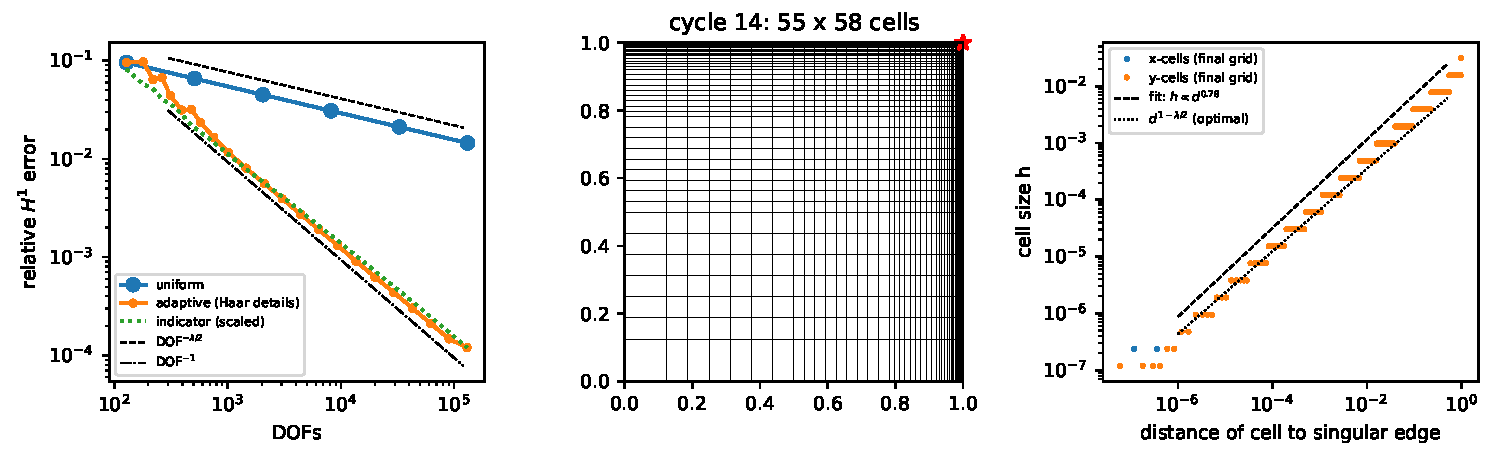
\includegraphics[width=\textwidth]{../figures/elasticity_corner.pdf}
\caption{Corner singularity with prescribed displacements. Left: error versus unknowns. Middle: grid
generated after 14 cycles (the star marks the singular point). Right: cell size versus distance to the
singular lines on the final grid.}\label{fig:elast}
\end{figure}

\subsection{Elastostatics with traction boundaries}
For the smooth solution, we impose tractions on one edge, on two adjacent edges (which creates a
traction--traction corner), or on two opposite edges. In every configuration, both the $H^1$ error and
the displacement on the traction edges converge at second order, and GMRES needs 18 to 27 iterations
independently of the grid size (Table~\ref{tab:tracsmooth}). With traction edges, the iteration counts
grow faster as $\nu\to\frac12$ (Table~\ref{tab:tracnu}).

\begin{table}[t]\centering\small
\caption{Traction boundaries, smooth solution: relative $H^1$ error for four configurations, GMRES
iterations, and maximum displacement error on the traction edges.}\label{tab:tracsmooth}
\begin{tabular}{r cc cc cc cc }
\toprule
 & \multicolumn{2}{c}{traction on T} & \multicolumn{2}{c}{traction on T+R} & \multicolumn{2}{c}{traction on L+B} & \multicolumn{2}{c}{traction on T+B}\\
$N$ & error & rate & error & rate & error & rate & error & rate\\
\midrule
16 & $3.30\times10^{-3}$ & -- & $4.31\times10^{-3}$ & -- & $3.89\times10^{-3}$ & -- & $5.99\times10^{-3}$ & --\\
32 & $8.20\times10^{-4}$ & 2.01 & $1.08\times10^{-3}$ & 2.00 & $9.70\times10^{-4}$ & 2.00 & $1.49\times10^{-3}$ & 2.01\\
64 & $2.05\times10^{-4}$ & 2.00 & $2.70\times10^{-4}$ & 2.00 & $2.42\times10^{-4}$ & 2.00 & $3.71\times10^{-4}$ & 2.00\\
128 & $5.11\times10^{-5}$ & 2.00 & $6.75\times10^{-5}$ & 2.00 & $6.05\times10^{-5}$ & 2.00 & $9.27\times10^{-5}$ & 2.00\\
256 & $1.28\times10^{-5}$ & 2.00 & $1.69\times10^{-5}$ & 2.00 & $1.51\times10^{-5}$ & 2.00 & $2.32\times10^{-5}$ & 2.00\\
\midrule
GMRES its & \multicolumn{2}{c}{18--20} & \multicolumn{2}{c}{27--27} & \multicolumn{2}{c}{26--27} & \multicolumn{2}{c}{18--20}\\
edge error ($N{=}256$) & \multicolumn{2}{c}{$8.64\times10^{-6}$} & \multicolumn{2}{c}{$1.84\times10^{-5}$} & \multicolumn{2}{c}{$1.09\times10^{-5}$} & \multicolumn{2}{c}{$1.53\times10^{-5}$}\\
\bottomrule
\end{tabular}

\end{table}
\begin{table}[t]\centering\small
\caption{Traction on two adjacent edges: dependence on Poisson's ratio.}\label{tab:tracnu}
\begin{tabular}{l ccc ccc}
\toprule
& \multicolumn{3}{c}{GMRES iterations} & \multicolumn{3}{c}{$e_{H^1}$}\\
$\nu$ & $N=32$ & $64$ & $128$ & $N=32$ & $64$ & $128$\\
\midrule
0.3 & 27 & 27 & 27 & $1.08{\times}10^{-3}$ & $2.70{\times}10^{-4}$ & $6.75{\times}10^{-5}$\\
0.4 & 33 & 33 & 33 & $1.93{\times}10^{-3}$ & $4.84{\times}10^{-4}$ & $1.21{\times}10^{-4}$\\
0.45 & 44 & 44 & 44 & $3.69{\times}10^{-3}$ & $9.29{\times}10^{-4}$ & $2.33{\times}10^{-4}$\\
0.49 & 102 & 98 & 98 & $1.75{\times}10^{-2}$ & $4.49{\times}10^{-3}$ & $1.13{\times}10^{-3}$\\
0.499 & 317 & 377 & 406 & $1.37{\times}10^{-1}$ & $4.15{\times}10^{-2}$ & $1.10{\times}10^{-2}$\\
\bottomrule
\end{tabular}

\end{table}
\begin{table}[t]\centering\small
\caption{One-dimensional model $u''=f$ with $u(0)$ and $u'(1)$ given: maximum error with an enhanced end
row of weight $\alpha$.}\label{tab:enh1d}
\begin{tabular}{r ccccc c}
\toprule
$\alpha$ & $N=32$ & $64$ & $128$ & $256$ & $512$ & rate\\
\midrule
$-1/12$ & $3.98\times10^{-4}$ & $1.02\times10^{-4}$ & $2.58\times10^{-5}$ & $6.49\times10^{-6}$ & $1.63\times10^{-6}$ & 2.00\\
0 (plain) & $1.18\times10^{-3}$ & $3.00\times10^{-4}$ & $7.58\times10^{-5}$ & $1.90\times10^{-5}$ & $4.77\times10^{-6}$ & 2.00\\
1/4 & $5.36\times10^{-3}$ & $1.36\times10^{-3}$ & $3.44\times10^{-4}$ & $8.62\times10^{-5}$ & $2.16\times10^{-5}$ & 2.00\\
1/2 & $9.54\times10^{-3}$ & $2.43\times10^{-3}$ & $6.11\times10^{-4}$ & $1.53\times10^{-4}$ & $3.84\times10^{-5}$ & 2.00\\
\bottomrule
\end{tabular}

\end{table}

Since pointwise traction conditions lose accuracy for isogeometric collocation on non-uniform
meshes~\cite{delorenzis2015isogeometric}, we repeated the smooth test on graded grids
(Table~\ref{tab:tracgraded}). The first family is the Chebyshev grid. The second is a geometric grid
graded toward the traction edge, with cell-size ratios up to 85. On both, the error remains second
order, and so does the displacement on the traction edges. On the strongly graded geometric grids,
however, the number of GMRES iterations grows with $N$, from 39 to 139, because the decoupled
preconditioner treats the traction rows only approximately.

\begin{table}[t]\centering\small
\caption{Traction on two adjacent edges, smooth solution, on graded grids.}\label{tab:tracgraded}
\begin{tabular}{r cccc cccc}
\toprule
 & \multicolumn{4}{c}{Chebyshev grid} & \multicolumn{4}{c}{geometric grid (toward traction edge)}\\
\cmidrule(lr){2-5}\cmidrule(lr){6-9}
$N$ & $e_{H^1}$ & rate & edge err. & its & $e_{H^1}$ & rate & $h_{\max}/h_{\min}$ & its\\
\midrule
16 & $6.73\times10^{-3}$ & -- & $8.10\times10^{-3}$ & 26 & $2.79\times10^{-2}$ & -- & 66 & 39\\
32 & $1.69\times10^{-3}$ & 1.99 & $2.04\times10^{-3}$ & 26 & $7.55\times10^{-3}$ & 1.89 & 76 & 50\\
64 & $4.23\times10^{-4}$ & 2.00 & $5.10\times10^{-4}$ & 26 & $1.93\times10^{-3}$ & 1.97 & 82 & 69\\
128 & $1.06\times10^{-4}$ & 2.00 & $1.27\times10^{-4}$ & 26 & $4.87\times10^{-4}$ & 1.99 & 85 & 139\\
\bottomrule
\end{tabular}

\end{table}

In the last elasticity test we place the square so that its top edge lies on a traction-free face of
the wedge, with the singular point at the end of that face. The exact traction on the top edge vanishes
to $10^{-14}$. This reproduces, on a single rectangle, the local situation at the re-entrant corner of the
L-shaped benchmark. Uniform grids reach $1.9\times10^{-2}$ with 132\,000 unknowns. Adaptive grids reach
$1.2\times10^{-4}$ with 149\,000 unknowns, at a fitted rate of $\mathrm{DOF}^{-1.00}$ and with 15 to 20
GMRES iterations (Table~\ref{tab:tracsing} and Fig.~\ref{fig:trac}).

\begin{table}[t]\centering\small
\caption{Singularity at the tip of a traction-free face: uniform versus automatic refinement.}\label{tab:tracsing}
\textit{(a) Uniform refinement}\\[2pt]
\begin{tabular}{rcc}
\toprule
unknowns & $e_{H^1}$ & GMRES its\\
\midrule
144 & $1.23{\times}10^{-1}$ & 18\\
544 & $8.45{\times}10^{-2}$ & 19\\
2112 & $5.80{\times}10^{-2}$ & 19\\
8320 & $3.97{\times}10^{-2}$ & 18\\
33024 & $2.72{\times}10^{-2}$ & 18\\
131584 & $1.87{\times}10^{-2}$ & 17\\
\bottomrule
\end{tabular}

\medskip
\textit{(b) Automatic refinement (Haar-detail indicator)}\\[2pt]
\begin{tabular}{rr ccc r}
\toprule
cycle & unknowns & $e_{H^1}$ & $h_{\min}$ & $\kappa(V)$ & GMRES its\\
\midrule
0 & 144 & $1.23{\times}10^{-1}$ & $1.2{\times}10^{-1}$ & 1.0 & 18\\
2 & 208 & $9.91{\times}10^{-2}$ & $3.1{\times}10^{-2}$ & 2.1 & 18\\
4 & 330 & $6.46{\times}10^{-2}$ & $1.6{\times}10^{-2}$ & 2.9 & 20\\
6 & 532 & $3.22{\times}10^{-2}$ & $3.9{\times}10^{-3}$ & 4.9 & 20\\
8 & 1040 & $1.53{\times}10^{-2}$ & $9.8{\times}10^{-4}$ & 6.7 & 20\\
10 & 2294 & $7.24{\times}10^{-3}$ & $2.4{\times}10^{-4}$ & 9.6 & 19\\
12 & 4982 & $3.42{\times}10^{-3}$ & $6.1{\times}10^{-5}$ & 13.2 & 18\\
14 & 11088 & $1.61{\times}10^{-3}$ & $1.5{\times}10^{-5}$ & 13.7 & 18\\
16 & 23320 & $7.60{\times}10^{-4}$ & $3.8{\times}10^{-6}$ & 18.4 & 17\\
18 & 48960 & $3.59{\times}10^{-4}$ & $9.5{\times}10^{-7}$ & 19.6 & 16\\
20 & 103008 & $1.70{\times}10^{-4}$ & $2.4{\times}10^{-7}$ & 26.1 & 16\\
21 & 149008 & $1.17{\times}10^{-4}$ & $1.2{\times}10^{-7}$ & 23.4 & 15\\
\bottomrule
\end{tabular}

\end{table}
\begin{figure}[t]\centering
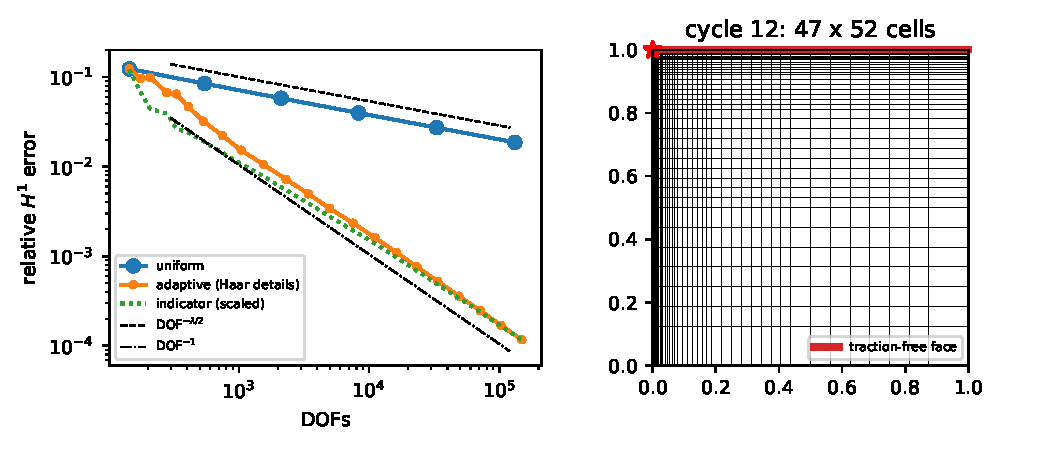
\includegraphics[width=0.8\textwidth]{../figures/elasticity_traction.pdf}
\caption{Singularity at the tip of a traction-free face (red edge; the star marks the singular point).
Left: error versus unknowns. Right: adaptive grid after 12 cycles.}\label{fig:trac}
\end{figure}

\subsection{Comparison with biquadratic finite elements}\label{sec:q2}
To place the elasticity results in context, we solve the traction-free-face problem with standard $Q_2$
(biquadratic Lagrange) Galerkin finite elements on exactly the same grids, both uniform and those
produced by the IHWC refinement loop. The $Q_2$ matrices are assembled exactly as Kronecker products of
one-dimensional matrices, and the implementation passes the patch test to $10^{-14}$. To separate the
effect of the discretization from that of the linear solver, we solve the $Q_2$ systems in two ways.
The first is a sparse direct solver (SuperLU). The second is the Galerkin counterpart of our own solver:
conjugate gradients preconditioned by fast diagonalization of
$(\lambda_L+2\mu)S_x\otimes M_y+\mu M_x\otimes S_y$ and of the corresponding $v$-operator, which
uses the generalized eigendecomposition of the one-dimensional stiffness and mass matrices.

Table~\ref{tab:q2} and Fig.~\ref{fig:q2} lead to three observations. On the same grid, $Q_2$ is about 1.3
times more accurate than IHWC, but it has about four times as many unknowns, because it places nodes at
cell corners, edge midpoints and cell centres. At equal numbers of unknowns, IHWC is therefore the more
accurate method; for example, it reaches $1.1\times10^{-3}$ with 16\,000 unknowns, where $Q_2$ reaches
$2.7\times10^{-3}$ with 19\,000. With equally efficient solvers, IHWC reaches a given accuracy roughly
twice as fast: $3.6\times10^{-4}$ in 0.13~s against $2.8\times10^{-4}$ in 0.24~s for $Q_2$, and
$1.2\times10^{-4}$ in 0.48~s against $9.2\times10^{-5}$ in 0.95~s. The sparse direct solver is one to two
orders of magnitude slower again (18.5~s at 194\,000 unknowns). Most of the speed advantage reported in
earlier comparisons of structured and unstructured methods is therefore a solver effect. The genuine
advantage of the discretization is the factor of about four in unknowns, and the resulting factor of
about two in time. Both methods recover the optimal adaptive rate on the IHWC-generated grids, and both
fast-diagonalization solvers need a mesh-independent number of iterations (11 to 20 for $Q_2$ with CG).

\begin{table}[t]\centering\small
\caption{IHWC collocation versus $Q_2$ finite elements on identical grids (traction-free-face
singularity; every third refinement cycle is shown). Times are solve times, excluding assembly and
setup.}\label{tab:q2}
\textit{(a) IHWC collocation: GMRES with the FDM preconditioner}\\[2pt]
\begin{tabular}{rr c ccc}
\toprule
cycle & unknowns & $e_{H^1}$ & setup (s) & solve (s) & MB\\
\midrule
0 & 144 & $1.23{\times}10^{-1}$ & 0.00 & 0.00 & 0.3\\
3 & 280 & $6.68{\times}10^{-2}$ & 0.00 & 0.01 & 0.4\\
6 & 532 & $3.22{\times}10^{-2}$ & 0.00 & 0.01 & 0.6\\
9 & 1550 & $1.05{\times}10^{-2}$ & 0.00 & 0.01 & 1.3\\
12 & 4982 & $3.42{\times}10^{-3}$ & 0.01 & 0.01 & 3.9\\
15 & 16182 & $1.11{\times}10^{-3}$ & 0.02 & 0.04 & 12.3\\
18 & 48960 & $3.59{\times}10^{-4}$ & 0.06 & 0.13 & 37.0\\
21 & 149008 & $1.17{\times}10^{-4}$ & 0.21 & 0.48 & 112.3\\
22 & 215644 & $8.03{\times}10^{-5}$ & 0.44 & 0.78 & 162.5\\
\bottomrule
\end{tabular}

\medskip
\textit{(b) $Q_2$ finite elements on the same grids, same cycles (rows) as in (a): CG with the FDM preconditioner, and sparse direct solve}\\[2pt]
\begin{tabular}{r c cccc}
\toprule
unknowns & $e_{H^1}$ & asm.\ (s) & CG (s) & MB & direct (s)\\
\midrule
480 & $7.22{\times}10^{-2}$ & 0.00 & 0.00 & 0.2 & 0.00\\
988 & $5.39{\times}10^{-2}$ & 0.01 & 0.00 & 0.3 & 0.00\\
1944 & $2.61{\times}10^{-2}$ & 0.01 & 0.00 & 0.7 & 0.02\\
5880 & $8.43{\times}10^{-3}$ & 0.02 & 0.01 & 2.0 & 0.06\\
19344 & $2.73{\times}10^{-3}$ & 0.04 & 0.03 & 6.8 & 0.51\\
63664 & $8.80{\times}10^{-4}$ & 0.13 & 0.09 & 22.7 & 3.08\\
193980 & $2.84{\times}10^{-4}$ & 0.39 & 0.32 & 69.4 & 20.49\\
592780 & $9.21{\times}10^{-5}$ & 1.54 & 1.19 & 212.6 & --\\
858676 & $6.33{\times}10^{-5}$ & 2.10 & 2.18 & 308.2 & --\\
\bottomrule
\end{tabular}

\end{table}
\begin{figure}[t]\centering
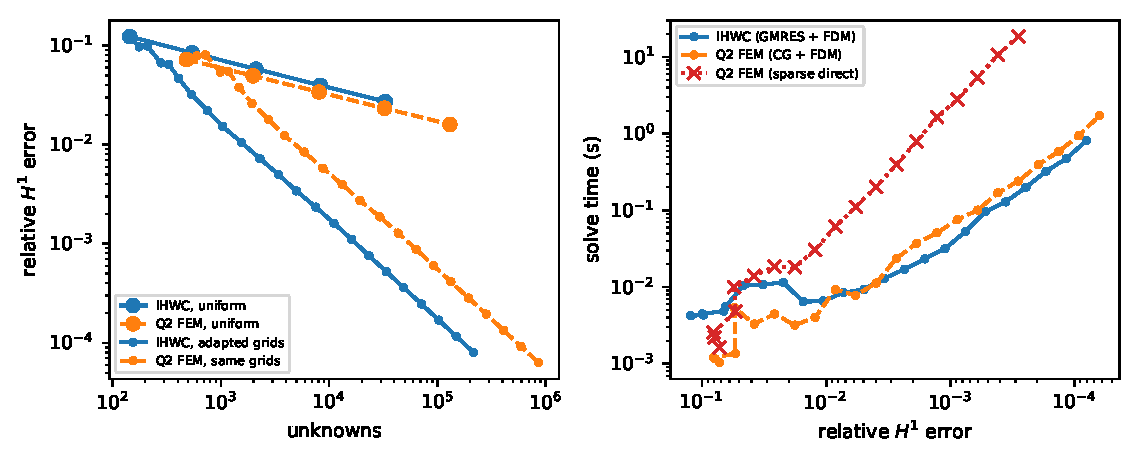
\includegraphics[width=0.9\textwidth]{../figures/ihwc_vs_q2.pdf}
\caption{IHWC collocation versus $Q_2$ finite elements on identical grids. Left: error versus number of
unknowns. Right: solve time versus error, for IHWC and for $Q_2$ with two solvers.}\label{fig:q2}
\end{figure}

\subsection{Phase-field verification}
For the Allen--Cahn shrinking circle with $\varepsilon=0.02$ and $R_0=0.3$, the sharp-interface limit
gives $R^2(t)=R_0^2-2\varepsilon^2t$. The grid-converged slope ($128^2$ and $256^2$ agree to four digits)
deviates from this law by 0.37\%, which is consistent with the $O(\varepsilon)$ corrections to that
limit. On the $64^2$ grid, the slope differs from the converged value by 1.35\% with $D_2$ and by 0.26\%
with $D_2^{(4)}$ (Table~\ref{tab:ac} and Fig.~\ref{fig:ac}). Both the modified and the original energy
decrease at every step.

\begin{table}[t]\centering\small
\caption{Allen--Cahn shrinking circle ($\varepsilon=0.02$, $\Delta t=0.05$): fitted slope, its deviation
from $-2\varepsilon^2$, and the largest step changes of the modified and the original energy.}\label{tab:ac}
\begin{tabular}{l cccc}
\toprule
run & fitted $\mathrm{d}R^2/\mathrm{d}t$ & rel.\ deviation from $-2\varepsilon^2$ & $\max_n(\tilde E^{n+1}-\tilde E^n)$ & $\max_n(E_h^{n+1}-E_h^n)$\\
\midrule
$N=64$, order 2 & $-8.14\times10^{-4}$ & 1.72\% & $-8.09\times10^{-6}$ & $-1.62\times10^{-4}$\\
$N=64$, order 4 & $-8.01\times10^{-4}$ & 0.11\% & $-7.91\times10^{-6}$ & $-1.58\times10^{-4}$\\
$N=128$, order 4 & $-8.03\times10^{-4}$ & 0.36\% & $-7.92\times10^{-6}$ & $-1.58\times10^{-4}$\\
$N=256$, order 4 & $-8.03\times10^{-4}$ & 0.37\% & $-7.92\times10^{-6}$ & $-1.58\times10^{-4}$\\
\bottomrule
\end{tabular}

\end{table}
\begin{figure}[t]\centering
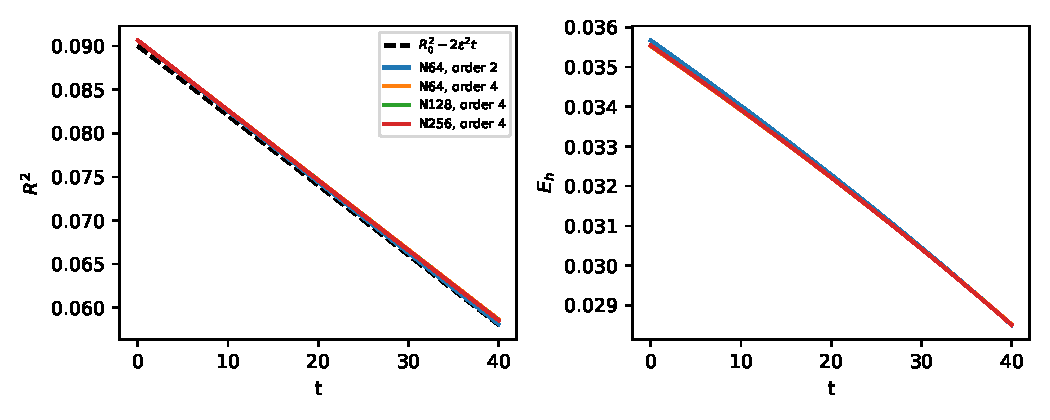
\includegraphics[width=0.72\textwidth]{../figures/allen_cahn_circle.pdf}
\caption{Allen--Cahn shrinking circle: $R^2(t)$ (left) and discrete energy (right).}\label{fig:ac}
\end{figure}

For a smooth Cahn--Hilliard solution ($\varepsilon=0.05$), grids with $N=18$, 54 and 162 are compared
with a grid with $N=486$. The factor of three between grids makes the coarse midpoints a subset of the
fine ones, so no interpolation is needed. The observed spatial orders are two for $D_2$ and four for
$D_2^{(4)}$ (Table~\ref{tab:chspace}), and the time order of SAV-BDF2 is two (Table~\ref{tab:chtime}).
For spinodal decomposition with $\varepsilon=0.01$ on $256^2$ and $\varepsilon=0.02$ on $96^3$, mass is
conserved to round-off and the energy decreases monotonically (Table~\ref{tab:spinodal},
Figs.~\ref{fig:spinodal} and~\ref{fig:ch3d}).

\begin{table}[t]\centering\small
\caption{Cahn--Hilliard: spatial self-convergence in the maximum norm.}\label{tab:chspace}
\begin{tabular}{r cc cc}
\toprule
 & \multicolumn{2}{c}{$D_2$} & \multicolumn{2}{c}{$D_2^{(4)}$}\\
$N$ & error & rate & error & rate\\
\midrule
18 & $7.95\times10^{-4}$ & -- & $1.36\times10^{-4}$ & --\\
54 & $9.32\times10^{-5}$ & 1.95 & $1.86\times10^{-6}$ & 3.91\\
162 & $9.40\times10^{-6}$ & 2.09 & $2.24\times10^{-8}$ & 4.02\\
\bottomrule
\end{tabular}

\end{table}
\begin{table}[t]\centering\small
\caption{Cahn--Hilliard: temporal convergence of SAV-BDF2 ($N=128$, $D_2^{(4)}$).}\label{tab:chtime}
\begin{tabular}{c cc}
\toprule
$\Delta t$ & error & rate\\
\midrule
$1.60{\times}10^{-4}$ & $8.12{\times}10^{-5}$ & --\\
$8.00{\times}10^{-5}$ & $2.05{\times}10^{-5}$ & 1.99\\
$4.00{\times}10^{-5}$ & $5.13{\times}10^{-6}$ & 1.99\\
$2.00{\times}10^{-5}$ & $1.29{\times}10^{-6}$ & 2.00\\
$1.00{\times}10^{-5}$ & $3.21{\times}10^{-7}$ & 2.00\\
\bottomrule
\end{tabular}

\end{table}
\begin{table}[t]\centering\small
\caption{Spinodal decomposition: conservation, energy and cost.}\label{tab:spinodal}
\begin{tabular}{l cc}
\toprule
 & 2D spinodal & 3D spinodal\\
\midrule
grid & $256^2$ & $96^3$\\
$\varepsilon$ & 0.01 & 0.02\\
steps & 5000+4500 & 1500\\
$\max_n|M_h^n-M_h^0|$ (with $M_h^0$) & $9.71\times10^{-17}$ (0.1) & $0.00\times10^{0}$ (0.1)\\
$\max_n(\tilde E^{n+1}-\tilde E^n)$ & $-3.31\times10^{-8}$ & $-4.79\times10^{-9}$\\
$\max_n(E_h^{n+1}-E_h^n)$ (sampled) & $-8.47\times10^{-7}$ & $-2.43\times10^{-7}$\\
$\xi=r/\sqrt{E_1+C}$ range & [1.000001, 1.000349] & --\\
CPU time/step (1 core) & 1.8 ms & 63 ms\\
\bottomrule
\end{tabular}

\end{table}
\begin{figure}[t]\centering
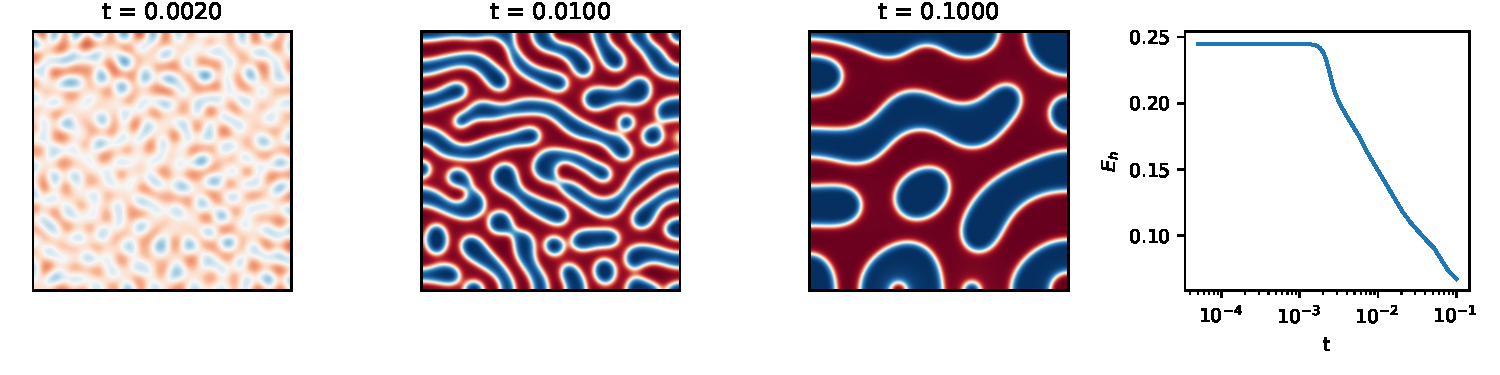
\includegraphics[width=\textwidth]{../figures/cahn_hilliard_spinodal.pdf}
\caption{Cahn--Hilliard spinodal decomposition on $256^2$: concentration at three times, and discrete energy.}\label{fig:spinodal}
\end{figure}
\begin{figure}[t]\centering
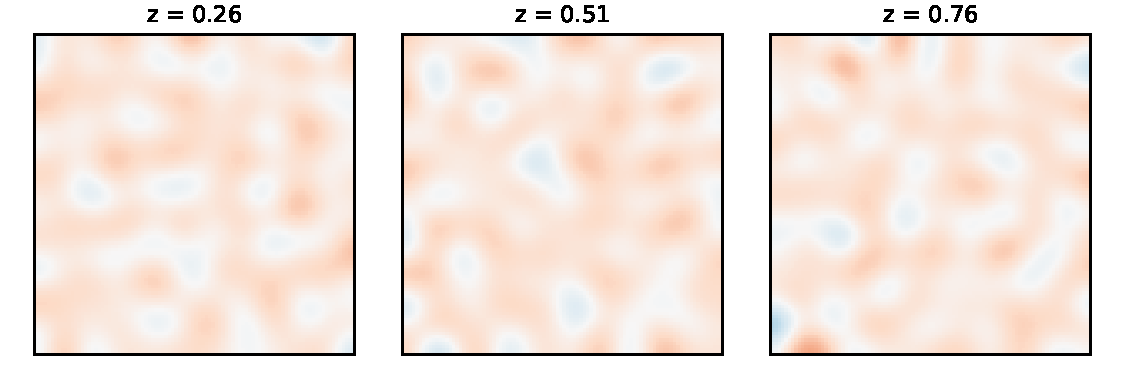
\includegraphics[width=0.62\textwidth]{../figures/cahn_hilliard_3d.pdf}
\caption{Three-dimensional Cahn--Hilliard on $96^3$: slices of the concentration at the final time.}\label{fig:ch3d}
\end{figure}

\subsection{Very sharp interfaces}\label{sec:sharp}
Phase-field computations in engineering often need interfaces that are as thin as possible relative to
the domain, and the practical question is how many grid nodes an interface needs. Across an interface,
$u\approx\tanh(d/\sqrt2\varepsilon)$. The profile goes from $-0.76$ to $0.76$ over a distance of
$2\sqrt2\varepsilon$, and its largest slope is $1/(\sqrt2\varepsilon)$. We therefore measure resolution in
nodes per $\sqrt2\varepsilon$.

To answer the question directly, we solve the steady planar interface
$u=\tanh((x-\frac12)/\sqrt2\varepsilon)$ on discrete grids. The interface is pinned at $x=\frac12$ by
symmetry, which removes its translation mode. Fig.~\ref{fig:res} and Table~\ref{tab:resolution} compare
the three-point finite-difference Laplacian with $D_2$ and $D_2^{(4)}$. The operator $D_2$ is about twice
as accurate as finite differences at every resolution, as Theorem~\ref{thm:fourth} predicts. The
corrected operator $D_2^{(4)}$ pays off from about 1.5 nodes per $\sqrt2\varepsilon$. At 3.6 nodes its
error is $1.7\times10^{-4}$, compared with $4.2\times10^{-3}$ for finite differences, a factor of 25. At
7.2 nodes it is $9.8\times10^{-6}$, compared with $1.1\times10^{-3}$, a factor of 110. Below about 1.4
nodes per $\sqrt2\varepsilon$ the interface is under-resolved, and $D_2^{(4)}$ is not better than $D_2$.

\begin{figure}[t]\centering
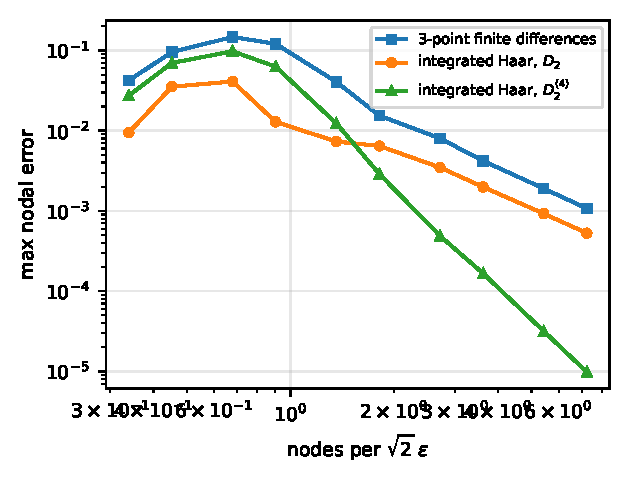
\includegraphics[width=0.5\textwidth]{../figures/interface_resolution.pdf}
\caption{Planar interface ($\varepsilon=0.01$): maximum nodal error versus nodes per $\sqrt2\varepsilon$.}\label{fig:res}
\end{figure}
\begin{table}[t]\centering\small
\caption{Planar interface ($\varepsilon=0.01$): maximum nodal error for three operators.}\label{tab:resolution}
\begin{tabular}{rr ccc}
\toprule
$N$ & nodes per $\sqrt2\varepsilon$ & 3-point FD & $D_2$ & $D_2^{(4)}$\\
\midrule
48 & 0.68 & $1.47{\times}10^{-1}$ & $4.10{\times}10^{-2}$ & $9.77{\times}10^{-2}$\\
64 & 0.91 & $1.21{\times}10^{-1}$ & $1.29{\times}10^{-2}$ & $6.29{\times}10^{-2}$\\
96 & 1.36 & $4.07{\times}10^{-2}$ & $7.32{\times}10^{-3}$ & $1.24{\times}10^{-2}$\\
128 & 1.81 & $1.54{\times}10^{-2}$ & $6.45{\times}10^{-3}$ & $2.89{\times}10^{-3}$\\
192 & 2.72 & $8.02{\times}10^{-3}$ & $3.48{\times}10^{-3}$ & $4.88{\times}10^{-4}$\\
256 & 3.62 & $4.20{\times}10^{-3}$ & $1.99{\times}10^{-3}$ & $1.66{\times}10^{-4}$\\
384 & 5.43 & $1.90{\times}10^{-3}$ & $9.23{\times}10^{-4}$ & $3.16{\times}10^{-5}$\\
512 & 7.24 & $1.07{\times}10^{-3}$ & $5.28{\times}10^{-4}$ & $9.78{\times}10^{-6}$\\
\bottomrule
\end{tabular}

\end{table}

For the Allen--Cahn six-fold star with $\varepsilon=0.004$, the initial interface
$r=0.25+0.08\cos6\theta$ evolves under curvature flow up to $t=120$, with $\Delta t=0.1$. A $1024^2$ run
with $D_2^{(4)}$, at 5.8 nodes per $\sqrt2\varepsilon$, serves as the reference. Coarse solutions are
compared with it at their own nodes through the exact cosine-series interpolant of the reference. On
$256^2$, which gives 1.45 nodes per $\sqrt2\varepsilon$, the high-curvature tips move visibly too slowly with
$D_2$, while $D_2^{(4)}$ follows the reference (Fig.~\ref{fig:star}). Table~\ref{tab:star} quantifies
this. $D_2^{(4)}$ on $256^2$ has an area error comparable to that of $D_2$ on $512^2$, with a quarter of
the unknowns, and on $512^2$ it is 16 times more accurate than $D_2$.

\begin{table}[t]\centering\small
\caption{Allen--Cahn star ($\varepsilon=0.004$): maximum nodal error and area error against the $1024^2$
reference, and cost per step.}\label{tab:star}
\begin{tabular}{l rcc c}
\toprule
run & unknowns & max error vs.\ ref. & area error & CPU time/step\\
\midrule
$256^2$, $D_2$ & 65536 & $1.36\times10^{-1}$ & $2.43\times10^{-4}$ & 1.6 ms\\
$256^2$, $D_2^{(4)}$ & 65536 & $5.27\times10^{-2}$ & $6.07\times10^{-5}$ & 1.4 ms\\
$512^2$, $D_2$ & 262144 & $4.12\times10^{-2}$ & $6.88\times10^{-5}$ & 9.5 ms\\
$512^2$, $D_2^{(4)}$ & 262144 & $2.63\times10^{-3}$ & $4.23\times10^{-6}$ & 8.6 ms\\
$1024^2$, $D_2^{(4)}$ (ref.) & 1048576 & -- & -- & 106 ms\\
\bottomrule
\end{tabular}

\end{table}
\begin{figure}[t]\centering
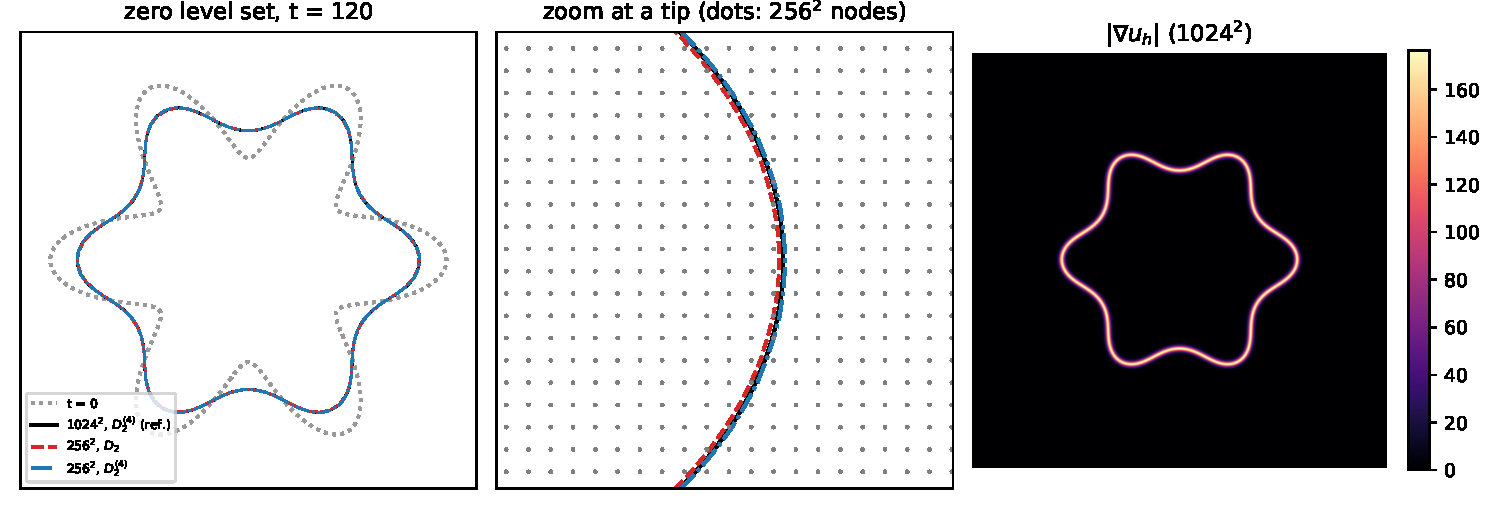
\includegraphics[width=\textwidth]{../figures/allen_cahn_star.pdf}
\caption{Allen--Cahn star, $\varepsilon=0.004$. Left: zero level sets at $t=0$ and $t=120$. Middle: zoom at
a tip, with the $256^2$ grid nodes. Right: gradient magnitude of the reference solution.}\label{fig:star}
\end{figure}

The most demanding case is Cahn--Hilliard with $\varepsilon=0.0015$ on a $1024^2$ grid. This gives only 2.2
nodes per $\sqrt2\varepsilon$, so that the whole interface, from $u=-0.76$ to $0.76$, spans about four
nodes. Starting from a random mixture, we use stabilized SAV ($S=4$) with three stages of 1500 steps each,
at $\Delta t=2\times10^{-7}$, $2\times10^{-6}$ and $2\times10^{-5}$, up to $t=0.033$. Mass is conserved to
$10^{-17}$, and both the modified and the original energy decrease at every step
(Table~\ref{tab:chsharp} and Fig.~\ref{fig:chsharp}). The largest value of $|u_h|$ stays below 1.03, so
there are no visible overshoots. The nodal profile across an interface coincides with the $\tanh$
profile, and the largest computed gradient, 467, matches the exact planar-interface value
$1/(\sqrt2\varepsilon)=471$. Table~\ref{tab:savstab} shows what happens without stabilization when the
computation is restarted at $t=0.0033$.

\begin{table}[t]\centering\small
\caption{Cahn--Hilliard with $\varepsilon=0.0015$ on $1024^2$, stabilized SAV ($S=4$).}\label{tab:chsharp}
\begin{tabular}{p{7.2cm} c}
\toprule
quantity & value\\
\midrule
grid and $\varepsilon$ & $1024^2$, 0.0015\\
nodes per $\sqrt2\varepsilon$ & 2.17\\
time steps & 1500$\times$$2{\times}10^{-7}$, 1500$\times$$2{\times}10^{-6}$, 1500$\times$$2{\times}10^{-5}$\\
largest mass deviation & $6.49{\times}10^{-18}$\\
largest step change of the modified energy & $-7.20{\times}10^{-8}$\\
largest change of $E_h$ between samples & $-3.37{\times}10^{-5}$\\
largest $|\nabla u_h|$ / planar-interface value $1/(\sqrt2\varepsilon)$ & 467 / 471\\
largest $|u_h|$ & 1.028\\
CPU time per step (one core) & 101 ms\\
\bottomrule
\end{tabular}

\end{table}
\begin{table}[t]\centering\small
\caption{Plain ($S=0$) versus stabilized ($S=4$) SAV for $\varepsilon=0.0015$: 150 steps from $t=0.0033$.}\label{tab:savstab}
\begin{tabular}{cc cccc}
\toprule
$S$ & $\Delta t$ & $\max|u_h|$ & $E_h$ (start $\to$ end) & $\xi$ & max $\Delta\tilde E$\\
\midrule
0 & $2{\times}10^{-5}$ & 77.33 & 0.062 $\to$ 503.681 & -0.00003 & $-4.59{\times}10^{-5}$\\
0 & $5{\times}10^{-6}$ & 122.58 & 0.062 $\to$ 801.433 & -0.00002 & $-3.23{\times}10^{-5}$\\
4 & $2{\times}10^{-5}$ & 1.04 & 0.062 $\to$ 0.050 & 1.00002 & $-5.02{\times}10^{-5}$\\
4 & $5{\times}10^{-6}$ & 1.04 & 0.062 $\to$ 0.058 & 1.00000 & $-2.27{\times}10^{-5}$\\
\bottomrule
\end{tabular}

\end{table}
\begin{figure}[t]\centering
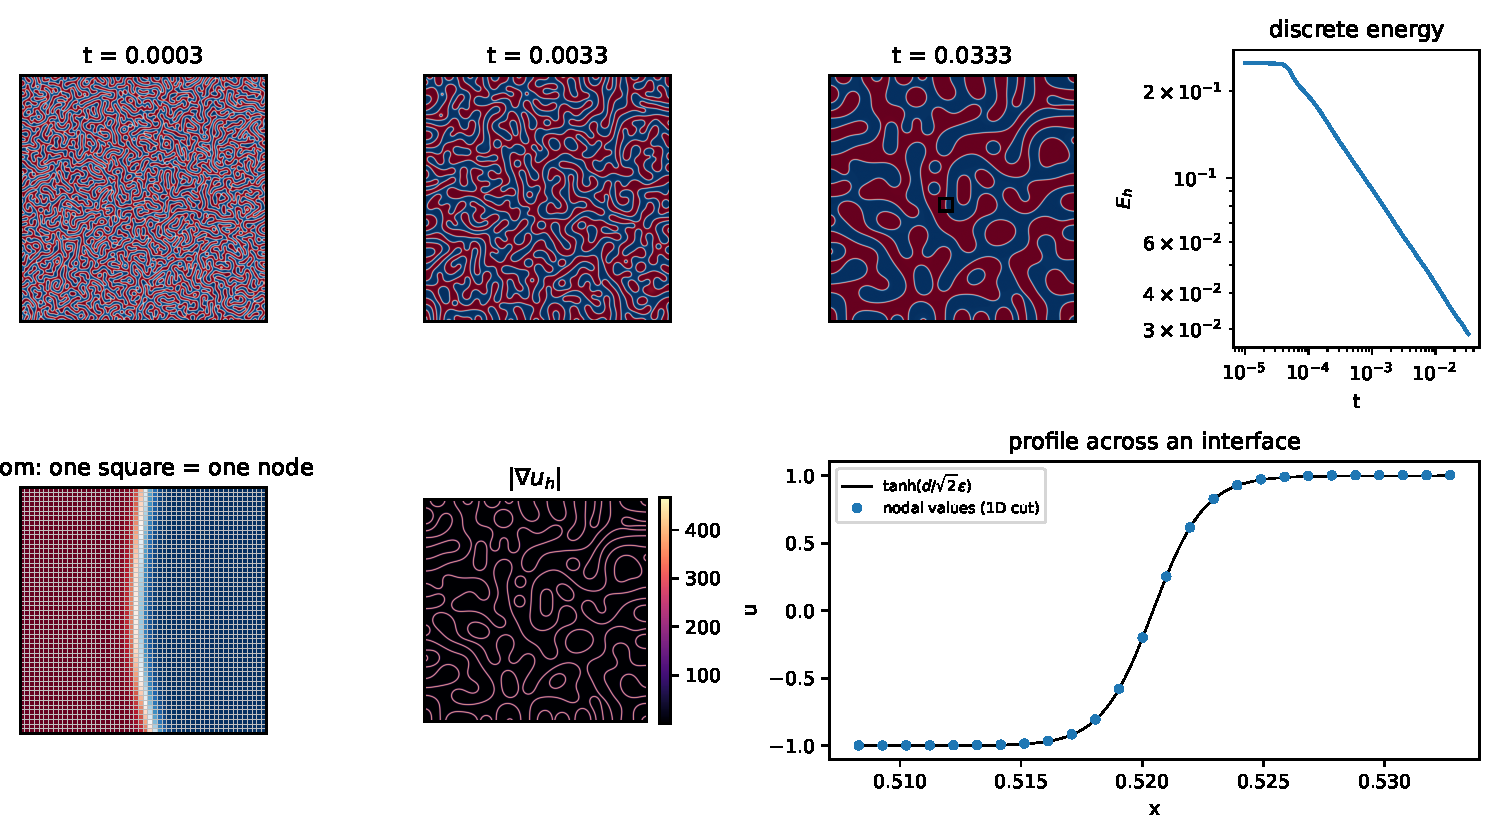
\includegraphics[width=\textwidth]{../figures/cahn_hilliard_sharp.pdf}
\caption{Cahn--Hilliard with $\varepsilon=0.0015$ on $1024^2$. Top: concentration at three times (the box
marks the zoomed region) and discrete energy. Bottom: zoom in which each square is one node; gradient
magnitude; nodal values along a grid line crossing an interface, compared with the $\tanh$ profile.}\label{fig:chsharp}
\end{figure}

\subsection{Comparison with other discretizations on uniform grids}\label{sec:compare}
All uniform-grid operators considered here are diagonalized by the same cosine transform. The
three-point difference, $D_2$, $D_2^{(4)}$, the compact Pad\'e operator and the cosine pseudo-spectral
operator therefore differ only in the eigenvalues used in Algorithm~2. This makes an exactly fair
comparison possible, with the same SAV scheme, the same time step and the same cost per step
(Table~\ref{tab:compare} and Fig.~\ref{fig:compare}). The operator $D_2$ is consistently about twice as
accurate as the three-point difference. The Pad\'e operator is about 1.4 times more accurate than
$D_2^{(4)}$, as predicted by the error constants. For problems on uniform boxes with zero-flux or periodic
conditions, the pseudo-spectral operator is far more accurate than all others. It reaches round-off on the
smooth Cahn--Hilliard case with $N=54$, and it is 15 times more accurate than $D_2^{(4)}$ on the $512^2$
star, with negligible overshoot ($|u|\le1.00003$).

We therefore do not advocate IHWC for phase-field problems on uniform boxes with zero-flux or periodic
conditions, where pseudo-spectral methods are the natural choice. The value of the formulation lies
elsewhere. It is a single structure-preserving discretization that also covers graded and adaptively
refined grids, prescribed values, traction conditions and singular solutions, where spectral methods do
not apply directly. It also offers the many existing HWCM codes a direct route to fast and provably
stable solvers.

\begin{table}[t]\centering\small
\caption{Uniform-grid operators within the identical SAV-BDF2 solver.}\label{tab:compare}
\begin{tabular}{l ccc cccc}
\toprule
 & \multicolumn{3}{c}{CH smooth, max error} & \multicolumn{4}{c}{AC star, $\varepsilon=0.004$}\\
\cmidrule(lr){2-4}\cmidrule(lr){5-8}
scheme & $N=18$ & $54$ & $162$ & error $256^2$ & error $512^2$ & area $256^2$ & area $512^2$\\
\midrule
3-point FD & $1.63\times10^{-3}$ & $1.89\times10^{-4}$ & $2.12\times10^{-5}$ & $3.89\times10^{-1}$ & $8.85\times10^{-2}$ & $6.02\times10^{-4}$ & $1.46\times10^{-4}$\\
IHWC $D_2$ & $7.96\times10^{-4}$ & $9.44\times10^{-5}$ & $1.06\times10^{-5}$ & $1.36\times10^{-1}$ & $4.12\times10^{-2}$ & $2.43\times10^{-4}$ & $6.88\times10^{-5}$\\
IHWC $D_2^{(4)}$ & $1.36\times10^{-4}$ & $1.86\times10^{-6}$ & $2.27\times10^{-8}$ & $5.27\times10^{-2}$ & $2.63\times10^{-3}$ & $6.07\times10^{-5}$ & $4.23\times10^{-6}$\\
compact 4th order (Pad\'e) & $9.42\times10^{-5}$ & $1.31\times10^{-6}$ & $1.60\times10^{-8}$ & $3.65\times10^{-2}$ & $1.78\times10^{-3}$ & $3.77\times10^{-5}$ & $2.88\times10^{-6}$\\
cosine pseudo-spectral & $4.40\times10^{-7}$ & $3.44\times10^{-15}$ & $1.61\times10^{-15}$ & $1.52\times10^{-2}$ & $1.68\times10^{-4}$ & $1.24\times10^{-5}$ & $2.72\times10^{-7}$\\
\bottomrule
\end{tabular}

\end{table}
\begin{figure}[t]\centering
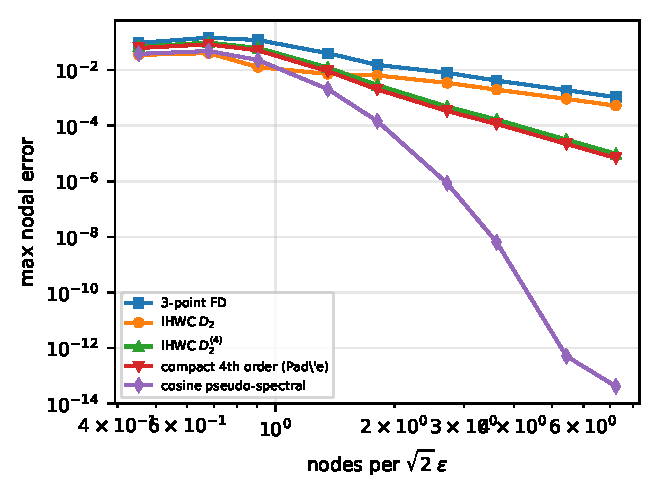
\includegraphics[width=0.5\textwidth]{../figures/scheme_comparison.pdf}
\caption{Planar interface: maximum nodal error versus resolution for five operators.}\label{fig:compare}
\end{figure}

\subsection{Performance}
Table~\ref{tab:perf} reports the time per Cahn--Hilliard step. On one CPU core, the cosine-transform
variant processes between $10^7$ and $3\times10^7$ unknowns per second. \todo{GPU columns pending; see the GPU section of the repository README.}


\begin{table}[t]\centering\small
\caption{Time per Cahn--Hilliard SAV-BDF2 step with $D_2^{(4)}$.}\label{tab:perf}
\textit{(a) CPU, double precision (ms per step)}\\[2pt]
\begin{tabular}{rr r cc}
\toprule
$d$ & $N$ & unknowns & GEMM & DCT\\
\midrule
2 & 128 & 16384 & 0.77 & 0.34\\
2 & 256 & 65536 & 2.25 & 1.55\\
2 & 512 & 262144 & 12.69 & 12.02\\
2 & 1024 & 1048576 & 146.23 & 103.26\\
2 & 2048 & 4194304 & -- & 363.06\\
3 & 32 & 32768 & 0.99 & 1.06\\
3 & 64 & 262144 & 8.11 & 9.41\\
3 & 128 & 2097152 & 191.31 & 189.90\\
\bottomrule
\end{tabular}

\medskip
\textit{(b) GPU (ms per step)}\\[2pt]
\begin{tabular}{rr cc cc}
\toprule
& & \multicolumn{2}{c}{double precision} & \multicolumn{2}{c}{single precision}\\
$d$ & $N$ & GEMM & DCT & GEMM & DCT\\
\midrule
2 & 128 & 1.10 & 2.13 & 1.18 & 2.17\\
2 & 256 & 3.14 & 2.59 & 3.29 & 2.18\\
2 & 512 & 13.98 & 2.89 & 11.21 & 2.88\\
2 & 1024 & 75.91 & 10.63 & 76.42 & 10.62\\
2 & 2048 & 589.88 & 44.33 & 591.10 & 44.18\\
3 & 32 & 1.46 & 2.93 & 1.80 & 2.94\\
3 & 64 & 3.35 & 3.66 & 3.42 & 3.63\\
3 & 128 & 35.14 & 31.91 & 34.97 & 32.05\\
\bottomrule
\end{tabular}

\end{table}

%==========================================================================
\section{Practical guidelines}\label{sec:guide}
%==========================================================================
Table~\ref{tab:guide} summarizes the choices that worked in our computations.

\begin{table}[t]\centering\small
\caption{Practical recommendations.}\label{tab:guide}
\begin{tabular}{p{3.3cm}p{10.6cm}}
\toprule
Decision & Recommendation\\
\midrule
Plain or corrected operator & Use $D_2^{(4)}$ for zero-flux or periodic problems, since it costs nothing extra. With general prescribed values, use $D_2$, because the correction does not raise the order there.\\
When not to use IHWC & For smooth or phase-field problems on uniform boxes with zero-flux or periodic conditions, a cosine pseudo-spectral operator is far more accurate at the same cost (Section~\ref{sec:compare}).\\
Interface resolution & Use at least 1.5 nodes per $\sqrt2\varepsilon$ with $D_2^{(4)}$. Expect a nodal error of about $10^{-3}$ at 2 to 3 nodes, and about $10^{-4}$ at 3.5 nodes (Table~\ref{tab:resolution}).\\
Time stepping (AC, CH) & Use SAV-BDF2 with stabilization $S\approx4$ and monitor $\xi=r/\sqrt{E_{1,h}+C}$; if it leaves $[0.999,1.001]$, reduce $\Delta t$. Start with small steps from random initial data, and increase $\Delta t$ as the structure coarsens, restarting with BDF1 at each change.\\
Solver & On uniform grids, use cosine or sine transforms. On graded grids, use fast diagonalization with dense matrix products (Theorem~\ref{thm:spectrum} guarantees that it applies). For coupled systems such as elasticity, use GMRES with the block preconditioner.\\
Adaptivity at singularities & Use the Haar-detail indicator with D\"orfler parameter $\theta\approx0.6$, a neighbour ratio of at most two, and an initial grid of $8\times8$ cells.\\
Traction conditions & Collocate tractions plainly at edge midpoints, without enhancement, and use the two normal-stress conditions at traction--traction corners.\\
Near incompressibility & Avoid $\nu>0.45$ with the present formulation (Tables~\ref{tab:nu} and~\ref{tab:tracnu}).\\
\bottomrule
\end{tabular}
\end{table}

%==========================================================================
\section{Limitations and outlook}\label{sec:limits}
%==========================================================================
The fast solvers require rectangular domains. Non-convex domains such as the full L-shaped domain, and
curved boundaries, need multi-patch coupling or geometry maps; the local corner structure of the L-shape
is, however, covered by the traction-free-face test. Tensor refinement extends refinement lines across the
whole domain. For point singularities this costs only a constant factor, and the optimal rate is retained.
For interfaces that move through the domain, local refinement would be preferable, but integrated Haar
functions are not compactly supported, so local refinement would require a different basis, such as
truncated hierarchical B-splines.

On the theoretical side, Theorem~\ref{thm:spectrum} guarantees real spectra on every grid, but the
conditioning of the eigenvectors is only observed, and the energy analysis of the phase-field schemes is
restricted to uniform grids, where $D_2$ is symmetric. The refinement indicator has no proved
reliability bound. In elasticity, the formulation loses robustness as $\nu\to\frac12$ and would need a
mixed displacement--pressure collocation in that regime. The comparison with $Q_2$ finite elements uses
the same solver class for both methods, but a comparison with adaptive hierarchical isogeometric
collocation~\cite{schillinger2013isogeometric} and with algebraic-multigrid-preconditioned finite elements
is still missing.

%==========================================================================
\section{Conclusions}
%==========================================================================
Rewritten in nodal form, Haar wavelet collocation is quadratic-spline collocation, and its
second-derivative operator is the product of two tridiagonal matrices with a real, simple and nonpositive
spectrum on every grid. This structural fact replaces the dense matrices of classical HWCM by fast tensor
solvers, gives a fourth-order correction at no cost, and supports provably mass-conserving and
energy-stable phase-field schemes. With stabilized SAV time stepping, Allen--Cahn and Cahn--Hilliard
interfaces are resolved accurately down to about two nodes per $\sqrt2\varepsilon$, at a cost of two fast
transforms per step. For elastostatics with prescribed displacements and tractions, preconditioned GMRES
converges in a mesh-independent number of iterations, and refinement driven by Haar detail coefficients
recovers the optimal rate at corner singularities. Against biquadratic finite elements with an equally
efficient solver, the method reaches a given accuracy with about a quarter of the unknowns and in about
half the time. For smooth problems on uniform boxes, pseudo-spectral methods remain the better choice.

\section*{Code and data availability}
The implementation, the unit tests, and the scripts that produce every table and figure of this paper
are available at \repo. Dependencies are listed in \texttt{requirements.txt} (CPU) and
\texttt{requirements-gpu.txt} (GPU, with CuPy).

\section*{Declaration of competing interest}
The author declares no known competing financial interests or personal relationships that could have
appeared to influence the work reported in this paper.

\clearpage
%==========================================================================
\appendix
\section{Proofs for Section~\ref{sec:method}}\label{app:ops}
%==========================================================================
\subsection{Theorem~\ref{thm:identity} and Corollary~\ref{cor:ops}}\label{app:identity}
\begin{proof}[Proof of Theorem~\ref{thm:identity}]
Let $\sigma_k=s'(t_k)$. On $I_k$, $s'(x)=\sigma_k+c_k(x-t_k)=\sigma_{k-1}+c_k(x-t_{k-1})$, hence
$\sigma_k-\sigma_{k-1}=c_kh_k$. Integrating $s'$ from $m_k$ to $m_{k+1}$ across $t_k$ gives
\[
U_{k+1}-U_k=\int_{m_k}^{t_k}\!\big(\sigma_k+c_k(x-t_k)\big)dx+\int_{t_k}^{m_{k+1}}\!\big(\sigma_k+c_{k+1}(x-t_k)\big)dx
=\sigma_kd_k-\frac{c_kh_k^2}{8}+\frac{c_{k+1}h_{k+1}^2}{8}.
\]
Dividing by $d_k$, subtracting the same relation for $k-1$, and using $\sigma_k-\sigma_{k-1}=c_kh_k$
gives~\eqref{eq:interior}. At the left end, $U_1-g_0=\sigma_0h_1/2+c_1h_1^2/8$, so
$2(U_1-g_0)/h_1=\sigma_0+c_1h_1/4$; subtracting this from the relation for $(U_2-U_1)/d_1$
gives~\eqref{eq:dirrow}. If $\sigma_0=0$, then $\sigma_1=c_1h_1$ and~\eqref{eq:neurow} follows. The right
end is analogous. The expressions for $s'(m_k)$ and for the end slopes follow from $s'=\sigma_0+\int s''$.
\end{proof}
\begin{proof}[Proof of Corollary~\ref{cor:ops}]
The off-diagonal entries of column $k$ of $A$ are positive and sum to $h_k^2/(8d_{k-1})+h_k^2/(8d_k)$, so
the column-dominance margin is $h_k-h_k^2/(4d_{k-1})-h_k^2/(4d_k)>0$, because $d_j>h_k/2$. For an end
column with a prescribed value the margin is $3h_1/4-h_1^2/(4d_1)>h_1/4$, and for a zero-slope end
column it is $h_1-h_1^2/(4d_1)>h_1/2$. With values prescribed at both ends, $L$ is a symmetric negative
definite three-point matrix, so $LU=Af-b_0g_0-b_1g_1$ has a unique solution.
\end{proof}

\subsection{Theorem~\ref{thm:spectrum}}\label{app:spectrum}
\begin{proof}
We use three standard facts~\cite{gantmacher2002oscillation,fallat2011totally}. (F1) A tridiagonal matrix
with nonnegative entries is totally nonnegative (all minors nonnegative) if and only if all its principal
minors are nonnegative. (F2) If $B$ is nonsingular and totally nonnegative, then $JB^{-1}J$ is totally
nonnegative, where $J=\mathrm{diag}((-1)^i)$; products of totally nonnegative matrices are totally
nonnegative (Cauchy--Binet). (F3) A totally nonnegative matrix is oscillatory if it is nonsingular and its
entries next to the diagonal are positive; the eigenvalues of an oscillatory matrix are real, positive and
simple (Gantmacher--Krein).

First let a value be prescribed at one or both ends. Then $-L$ is an irreducible tridiagonal matrix with
positive diagonal, negative off-diagonal entries, zero row sums in the interior and a positive row sum
in at least one end row. It is therefore a nonsingular M-matrix, and all its principal minors are positive.
The matrix $J(-L)J$ has the same principal minors and nonnegative entries, so it is totally nonnegative by
(F1). By (F2), $(-L)^{-1}=J\,(J(-L)J)^{-1}J$ is totally nonnegative; it is also entrywise positive, as the
inverse of an irreducible M-matrix. The matrix $A$ has nonnegative entries, and $JAJ$ is a Z-matrix that is
strictly diagonally dominant by columns (Corollary~\ref{cor:ops}), hence an M-matrix. Its principal minors,
which are those of $A$, are therefore positive, and $A$ is totally nonnegative by (F1). The product
$P=(-L)^{-1}A$ is totally nonnegative and nonsingular, and it is entrywise positive, since $(-L)^{-1}$ is
entrywise positive and $A$ is nonnegative with a positive diagonal. By (F3), $P$ is oscillatory and has $N$
real, positive, simple eigenvalues. Since $D_2=A^{-1}L=-P^{-1}$, the eigenvalues of $D_2$ are real,
negative and simple.

If the slope vanishes at both ends, $L$ is singular. Let
$0<\sigma<8/\max_kh_k^2$, and consider $-(L-\sigma A)=-L+\sigma A$. Its off-diagonal entries are
$-1/d_k+\sigma h^2/(8d_k)<0$, and its columns have positive dominance margin $\sigma h_k$, because the columns
of $L$ sum to zero and those of $A$ sum to $h_k$ (Proposition~\ref{prop:mass}). It is therefore a nonsingular
M-matrix, and the argument above applies to $(-L+\sigma A)^{-1}A$. Hence $A^{-1}L-\sigma I$ has real,
negative, simple eigenvalues, so the eigenvalues of $D_2$ are real, simple and smaller than $\sigma$. Since
$\sigma$ can be arbitrarily small, they are nonpositive, and the constant vector spans the kernel.
\end{proof}

\subsection{Proposition~\ref{prop:uniform}}\label{app:uniform}
\begin{proof}
With $h_k=h$ we have $d_k=h$, and the coefficients of~\eqref{eq:interior}--\eqref{eq:neurow} become
$h(\frac18,\frac68,\frac18)$, $h(\frac58,\frac18)$ and $h(\frac78,\frac18)$. These are the rows of
$h(I+\delta^2/8)$, while the left-hand sides are the rows of $\delta^2/h$. Since $I+\delta^2/8$ is a
polynomial in the symmetric matrix $\delta^2$, the two commute, and $D_2=h^{-2}(I+\delta^2/8)^{-1}\delta^2$ is
symmetric. The end rows of $\delta^2$ correspond to ghost values $U_0=-U_1$ (odd reflection) or $U_0=U_1$
(even reflection), whose eigenvectors are the DST-II and DCT-II vectors with eigenvalues $\mu_k\in[-4,0]$.
Finally, $\mu\mapsto8\mu/(8+\mu)$ maps $[-4,0]$ monotonically onto $[-8,0]$.
\end{proof}

\subsection{Theorem~\ref{thm:fourth}}\label{app:fourth}
\begin{proof}
By the reflection property, the zero-slope matrices act on $U$ in the same way as the circulant matrices
of the $2N$-point periodic grid act on the even extension. For a sampled exponential $e^{i\omega x}$, the
circulant $D_2$ has the eigenvalue $\lambda(\omega h)/h^2$, with the $2\pi$-periodic analytic symbol
$\lambda(\theta)=8\mu/(8+\mu)$, where $\mu=-4\sin^2(\theta/2)=-\theta^2+\theta^4/12+O(\theta^6)$. Hence
$\lambda=\mu-\mu^2/8+O(\mu^3)=-\theta^2-\theta^4/24+O(\theta^6)$, which gives the first statement mode by
mode. The symbol of $D_2^{(4)}$ is $\lambda+\lambda^2/24=-\theta^2+O(\theta^6)$, so
$|\lambda_4(\omega h)/h^2+\omega^2|\le Ch^4\omega^6$ for $|\omega h|\le\pi$. For $|\omega h|>\pi$ the bound
holds trivially, because $|\lambda_4|\le16/3$. Summing over the rapidly decaying Fourier coefficients of
the smooth periodic extension gives the $O(h^4)$ bound. The spectral statement follows because
$\lambda+h^2\lambda^2/24\le0$ for $\lambda\in[-24/h^2,0]$. Prescribed values with odd extensions are
treated in the same way.
\end{proof}

\subsection{Proposition~\ref{prop:mass}}\label{app:mass}
\begin{proof}
From~\eqref{eq:interior} and~\eqref{eq:neurow}, column $k$ of $A$ sums to
$h_k-\frac{h_k^2}{8d_{k-1}}-\frac{h_k^2}{8d_k}+\frac{h_k^2}{8d_{k-1}}+\frac{h_k^2}{8d_k}=h_k$, that is,
$\mathbf 1^{\mathsf T}A=h^{\mathsf T}$. Hence $h^{\mathsf T}D_2=\mathbf 1^{\mathsf T}L=0$, because the columns of
the zero-slope difference matrix sum to zero. On uniform grids, $\int_{I_k}s=hU_k+h^3c_k/24$ exactly, and
$\sum_kh\,c_k=s'(b)-s'(a)=0$.
\end{proof}

%==========================================================================
\section{Proof of Theorem~\ref{thm:energy}}\label{app:energy}
%==========================================================================
\begin{proof}
For solvability, eliminating $\mu$ gives $Mu^{n+1}=g+2\Delta t\,S\,G_h\bar u-2\Delta t\,r^{n+1}G_h\bar b$
with $M=3I+2\Delta t\,G_h(\varepsilon^2K+SI)$. The matrix $M$ is symmetric positive definite, because $G_h$
and $K$ commute and are positive semidefinite. Writing $u^{n+1}=p+r^{n+1}q$ and substituting
into~\eqref{eq:sav2} gives a scalar equation for $r^{n+1}$ whose coefficient is
$3-\tfrac32\langle\bar b,q\rangle_h\ge3$, since
$\langle\bar b,q\rangle_h=-2\Delta t\langle\bar b,M^{-1}G_h\bar b\rangle_h\le0$.

For mass conservation in CH, $\langle K\mu,1\rangle_h=\langle\mu,K1\rangle_h=0$, so
$\langle3u^{n+1}-4u^n+u^{n-1},1\rangle_h=0$. Since the BDF1 first step also conserves mass, induction gives
conservation, and Proposition~\ref{prop:mass} identifies the discrete sum with the integral.

For the energy, take the inner product of~\eqref{eq:sav1} with $2\Delta t\,\mu^{n+1}$. The left-hand side
gives $-2\Delta t\langle G_h\mu,\mu\rangle_h\le0$. On the right-hand side, write $a=u^{n+1}$, $b=u^n$ and
$c=u^{n-1}$, and use the identities
\begin{align*}
2\langle3a-4b+c,Ka\rangle_h&=\|a\|_K^2-\|b\|_K^2+\|2a-b\|_K^2-\|2b-c\|_K^2+\|a-2b+c\|_K^2,\\
\langle3a-4b+c,a-2b+c\rangle_h&=\|a-b\|_h^2-\|b-c\|_h^2+2\|a-2b+c\|_h^2,
\end{align*}
the second of which follows from $(3x-y)(x-y)=x^2-y^2+2(x-y)^2$ with $x=a-b$ and $y=b-c$, together with
the scalar version of the first identity applied to~\eqref{eq:sav2} multiplied by $2r^{n+1}$. Collecting
terms gives
\begin{multline*}
\tilde E^{n+1}-\tilde E^n=-\Delta t\langle G_h\mu^{n+1},\mu^{n+1}\rangle_h-\tfrac{\varepsilon^2}{4}\|a-2b+c\|_K^2\\
-\tfrac12(r^{n+1}-2r^n+r^{n-1})^2-S\|a-2b+c\|_h^2\le0.
\end{multline*}
The same argument applies to BDF1 and to both $D_2$ and $D_2^{(4)}$, since it uses only the symmetry and
semidefiniteness of $K$ in $\langle\cdot,\cdot\rangle_h$ (Proposition~\ref{prop:uniform} and
Theorem~\ref{thm:fourth}).
\end{proof}

%==========================================================================
\begin{thebibliography}{99}
\bibitem{chen1997haar} C.F. Chen, C.H. Hsiao, Haar wavelet method for solving lumped and distributed-parameter systems, IEE Proc. Control Theory Appl. 144 (1997) 87--94.
\bibitem{lepik2005numerical} \"U. Lepik, Numerical solution of differential equations using Haar wavelets, Math. Comput. Simul. 68 (2005) 127--143.
\bibitem{lepik2007application} \"U. Lepik, Application of the Haar wavelet transform to solving integral and differential equations, Proc. Estonian Acad. Sci. Phys. Math. 56 (2007) 28--46.
\bibitem{lepik2011solving} \"U. Lepik, Solving PDEs with the aid of two-dimensional Haar wavelets, Comput. Math. Appl. 61 (2011) 1873--1879.
\bibitem{lepik2014book} \"U. Lepik, H. Hein, Haar Wavelets: With Applications, Springer, Cham, 2014.
\bibitem{majak2015accuracy} J. Majak, B. Shvartsman, K. Karjust, M. Mikola, A. Haavaj\~oe, M. Pohlak, On the accuracy of the Haar wavelet discretization method, Compos. B Eng. 80 (2015) 321--327.
\bibitem{majak2015convergence} J. Majak, B.S. Shvartsman, M. Kirs, M. Pohlak, H. Herranen, Convergence theorem for the Haar wavelet based discretization method, Compos. Struct. 126 (2015) 227--232.
\bibitem{majak2018higher} J. Majak, M. Pohlak, K. Karjust, M. Eerme, J. Kurnitski, B.S. Shvartsman, New higher order Haar wavelet method: Application to FGM structures, Compos. Struct. 201 (2018) 72--78.
\bibitem{ratas2021solving} M. Ratas, J. Majak, A. Salupere, Solving nonlinear boundary value problems using the higher order Haar wavelet method, Mathematics 9 (2021) 2809.
\bibitem{dubeau2004nonuniform} F. Dubeau, S. Elmejdani, R. Ksantini, Non-uniform Haar wavelets, Appl. Math. Comput. 159 (2004) 675--693.
\bibitem{lepik2008nonuniform} \"U. Lepik, Solving integral and differential equations by the aid of non-uniform Haar wavelets, Appl. Math. Comput. 198 (2008) 326--332.
\bibitem{oruc2019nonuniform} \"O. Oru\c{c}, A non-uniform Haar wavelet method for numerically solving two-dimensional convection-dominated equations and two-dimensional near singular elliptic equations, Comput. Math. Appl. 77 (2019) 1799--1820.
\bibitem{houstis1988quadratic} E.N. Houstis, C.C. Christara, J.R. Rice, Quadratic-spline collocation methods for two-point boundary value problems, Int. J. Numer. Methods Eng. 26 (1988) 935--952.
\bibitem{christara1994quadratic} C.C. Christara, Quadratic spline collocation methods for elliptic partial differential equations, BIT 34 (1994) 33--61.
\bibitem{christara2006optimal} C.C. Christara, K.S. Ng, Optimal quadratic and cubic spline collocation on nonuniform partitions, Computing 76 (2006) 227--257.
\bibitem{christara2006adaptive} C.C. Christara, K.S. Ng, Adaptive techniques for spline collocation, Computing 76 (2006) 259--277.
\bibitem{christara2002fast} C.C. Christara, K.S. Ng, Fast Fourier transform solvers and preconditioners for quadratic spline collocation, BIT 42 (2002) 702--739.
\bibitem{auricchio2010isogeometric} F. Auricchio, L. Beir\~ao da Veiga, T.J.R. Hughes, A. Reali, G. Sangalli, Isogeometric collocation methods, Math. Models Methods Appl. Sci. 20 (2010) 2075--2107.
\bibitem{schillinger2013isogeometric} D. Schillinger, J.A. Evans, A. Reali, M.A. Scott, T.J.R. Hughes, Isogeometric collocation: Cost comparison with Galerkin methods and extension to adaptive hierarchical NURBS discretizations, Comput. Methods Appl. Mech. Engrg. 267 (2013) 170--232.
\bibitem{anitescu2015isogeometric} C. Anitescu, Y. Jia, Y.J. Zhang, T. Rabczuk, An isogeometric collocation method using superconvergent points, Comput. Methods Appl. Mech. Engrg. 284 (2015) 1073--1097.
\bibitem{gomez2016variational} H. Gomez, L. De Lorenzis, The variational collocation method, Comput. Methods Appl. Mech. Engrg. 309 (2016) 152--181.
\bibitem{delorenzis2015isogeometric} L. De Lorenzis, J.A. Evans, T.J.R. Hughes, A. Reali, Isogeometric collocation: Neumann boundary conditions and contact, Comput. Methods Appl. Mech. Engrg. 284 (2015) 21--54.
\bibitem{lynch1964direct} R.E. Lynch, J.R. Rice, D.H. Thomas, Direct solution of partial difference equations by tensor product methods, Numer. Math. 6 (1964) 185--199.
\bibitem{bartels1972solution} R.H. Bartels, G.W. Stewart, Solution of the matrix equation $AX+XB=C$, Commun. ACM 15 (1972) 820--826.
\bibitem{sangalli2016isogeometric} G. Sangalli, M. Tani, Isogeometric preconditioners based on fast solvers for the Sylvester equation, SIAM J. Sci. Comput. 38 (2016) A3644--A3671.
\bibitem{shen2018scalar} J. Shen, J. Xu, J. Yang, The scalar auxiliary variable (SAV) approach for gradient flows, J. Comput. Phys. 353 (2018) 407--416.
\bibitem{gantmacher2002oscillation} F.R. Gantmacher, M.G. Krein, Oscillation Matrices and Kernels and Small Vibrations of Mechanical Systems, revised ed., AMS Chelsea Publishing, Providence, RI, 2002.
\bibitem{fallat2011totally} S.M. Fallat, C.R. Johnson, Totally Nonnegative Matrices, Princeton University Press, Princeton, NJ, 2011.
\bibitem{dorfler1996convergent} W. D\"orfler, A convergent adaptive algorithm for Poisson's equation, SIAM J. Numer. Anal. 33 (1996) 1106--1124.
\bibitem{williams1952stress} M.L. Williams, Stress singularities resulting from various boundary conditions in angular corners of plates in extension, J. Appl. Mech. 19 (1952) 526--528.
\bibitem{grisvard1985elliptic} P. Grisvard, Elliptic Problems in Nonsmooth Domains, Pitman, Boston, 1985.
\bibitem{babuska1979direct} I. Babu\v{s}ka, R.B. Kellogg, J. Pitk\"aranta, Direct and inverse error estimates for finite elements with mesh refinements, Numer. Math. 33 (1979) 447--471.
\bibitem{apel1999anisotropic} T. Apel, Anisotropic Finite Elements: Local Estimates and Applications, Teubner, Stuttgart, 1999.
\end{thebibliography}

\end{document}
